\documentclass{UoNMCHA}
\usepackage[authoryear]{natbib}
\usepackage{array,booktabs} % For nice tables
\usepackage{amsmath,amsfonts,amssymb} % For nice maths
\usepackage{color,mathtools}
\usepackage{enumerate,tensor}
\usepackage{listings}
\usepackage{subfig}
\usepackage{multicol}
\usepackage{hyperref}
\usepackage{float}
\usepackage[mathscr]{euscript}
\usepackage[parfill]{parskip}   % For replacing paragraph indenting with a newline instead
\usepackage{enumitem}

% Number equations per section
\numberwithin{equation}{section}

\hypersetup{
%    bookmarks=true,         % show bookmarks bar?
%    unicode=false,          % non-Latin characters in AcrobatÕs bookmarks
%    pdftoolbar=true,        % show AcrobatÕs toolbar?
%    pdfmenubar=true,        % show AcrobatÕs menu?
%    pdffitwindow=false,     % window fit to page when opened
%    pdfstartview={FitH},    % fits the width of the page to the window
%    pdftitle={My title},    % title
%    pdfauthor={Author},     % author
%    pdfsubject={Subject},   % subject of the document
%    pdfcreator={Creator},   % creator of the document
%    pdfproducer={Producer}, % producer of the document
%    pdfkeywords={keyword1} {key2} {key3}, % list of keywords
%    pdfnewwindow=true,      % links in new window
    colorlinks=true,       % false: boxed links; true: colored links
    linkcolor=blue,          % color of internal links
    citecolor=blue,        % color of links to bibliography
%    filecolor=magenta,      % color of file links
    urlcolor=blue           % color of external links
}

\definecolor{MATLABKeyword}{rgb}{0,0,1}
\definecolor{MATLABComment}{rgb}{0.1328125,0.54296875,0.1328125}
\definecolor{MATLABString}{rgb}{0.625,0.125,0.9375}

\lstset{language=Matlab,
    basicstyle=\small\ttfamily,
    keywordstyle=\color{MATLABKeyword},
    %identifierstyle=,
    commentstyle=\color{MATLABComment},
    stringstyle=\color{MATLABString},
    numberstyle=\tiny,
    %numbers=left,
    basewidth=0.5em}

\firstpage{1}    % Set page number for first page
\UoNMCHAreportNo{Final Year Project} %Report number
\UoNMCHAyear{2019}   % Year\\
\shorttitle{Vision-Based Control of an Industrial Robot Arm} %For odd pages
%%%%%%%%%%%%%%%%%%%%%%%%%%%%%%%%%%%%%%%%%%%%%%%%%%%%
\begin{document}
\title{Vision-Based Control of Industrial Robot Arm \\ \ \\
{\small Final Year Project Report for MECH4841  \\July 2020}}
\author[UoNMCHA]{Muhammad Hasham Khan}
\address[UoNMCHA]{
Student of Mechatronics Engineering,\\
The University of Newcastle, Callaghan, NSW 2308, AUSTRALIA \\
Student Number: 3256011 \\
E-mail: \href{mailto:Muhammad.H.Khan@uon.edu.au}{\textsf{Muhammad.H.Khan@uon.edu.au}}}
%%%%%%%%%%%%%%%%%%%%%%%%%%%%%%%%%%%
\maketitle
\onecolumn

%%%%%%%%%%%%%%%%%%%%%%%%%%%%%%%%%%%%
\vspace{-5mm}
\section*{Dot Point Summary}
%\vspace{mm}

This project explores:
\begin{itemize}
	\item Modelling and controlling a robotic manipulator
	\item Camera modelling and feature point extraction
	\item Training a machine learning based object detector
	\item Deriving a visual-servoing controller 
	\item Experimentally validating the previous dot points on hardware 
	\item Integrating these different subsystems together to demonstrate a pick-and-place task using visual-servoing on a robotic manipulator.

\end{itemize}

\newpage
\vspace{-5mm}
\section*{Abstract}

Vision-based control allows robots to shift from structured to dynamic environments by using the substantial information obtained through visual sensors. \
This technique has vast applications in robot navigation, localisation and control.\ This method is explored by implementing a solution for
a \textit{pick-and-place} task using a 5DOF robotic manipulator in a eye-in-hand configuration. This problem is extended to include sorting between different target objects. \

The task was successfully demonstrated using image based visual servoing and allowed alignment of feature points with an accuracy of \textit{20} pixels.
A robust faster region-based convolutional neural network was also trained to reliably detect target objects. The modular structure of this work allows it to form the basis of further research. \ 

Future improvements include incorporating dynamic models, investigating uncalibrated visual servoing, exploring the use of different camera configurations and applying this work on a ABB IRB-120 industrial robot arm.

%%%%%%%%%%%%%%
\newpage
\vspace{-2mm}
\section*{Acknowledgements}

Thank you to:
\begin{itemize}
	\item My supervisor, Alejandro Donaire, for all his guidance, support and enthusiasm throughout my project.
	\item Ampcontrol CSM for providing a platform to implement my work in an industrial environment
	\item Dr Chris Renton for his standout coursework that inspired my understanding and appreciation of robotics
	\item My family and friends for bearing with my prolonged absences
	\item All the mechatronics boys for their camaraderie
	
\end{itemize}

%%%%%%%%%%%%%%%%%%%%%%%%%%%%%
\newpage
\tableofcontents
\listoffigures
\listoftables
\newpage
%%%%%%%%%%%%%%%%%%%%%%%%%%%%%%%
\section{Introduction}

Advances in control theory have been leveraged to perform repetitive and dangerous tasks. In this context, robots have been implemented to drastically increase productivity in manufacturing. Unlike human workers, machines have typically been limited to structured environments, such as well-defined factory floors, due to the current limitations of robotic environmental awareness. Providing robots with situational awareness and intelligent decision-making capabilities allows them to operate in dynamic environments that traditional methods cannot match.  The use of visual feedback techniques is a key asset in this objective. \

\textit{Visual feedback} relies on perceiving and responding to optical information. Controlling a robot using visual data follows naturally from how we use our vision system to gather information from, and interact with, the world around us. Artificial neural networks take inspiration from this system, mimicking the learning capabilities of our brain by recognising environmental markers. In this way, visual-servoing controllers can perform hand-eye coordination tasks. By exploring visual control, robots are becoming smarter. \

This project explores visual control in the context of robotic manipulators. A common task in industry is picking up objects and placing them at a desired location. This is known as a \textit{pick-and-place} task and is typically achieved by constraining a target object at a set position in space. Then the robot arm moves its grasping tool to a set position and successfully manipulates the object. \

This relies on a key assumption; \textbf{the object must be exactly where the robot expects it to be} \citep{corke2017robotics}. In the real word, this is rarely guaranteed without the use of expensive jigs and conveyers and requires recalibration each time the object or robot is moved from their original position. \

Visual feedback control, commonly known as visual servoing, overcomes these limitations and is therefore the focus of this project. This is highlighted in Appendix \ref{Industrial Application}, where an example of visual servoing being used in industry is showcased. The remainder of this section defines in detail the problem, a brief literature review on how others approached the task and the method developed to overcome this limitation. 

    
    
    \subsection{Objective}\label{Objective}
%    \item \textbf{Problem}: Describe the specifics of the problem you are trying to address
    
   The goal of this project is to use a robotic manipulator with an eye-in-hand camera to implement a pick-and-place task. Additionally, the manipulator must be able to sort between different objects and only grasp the desired one.\
	
	This task has a broad scope and various assumptions were made for simplification.
	
	\subsection{Assumptions} \label{Assumptions}
    
    The following assumptions were made during this project:\\
    \begin{description}[style=multiline,leftmargin=3cm]
    	\item[\textbf{Assumption A}:] The robot arm is fixed and stationary.
    	\item[\textbf{Assumption B}:] The robot arm has a in-built joint controller. It can, through an interface, prescribe desired joint angles.
    	\item[\textbf{Assumption C}:] The desired objects to be picked are uniform and their geometry is known. Additionally, they will be differentiable by some visual indicator.
    	\item[\textbf{Assumption D}:] The robot arm and desired objects will be located on a planar workspace free of obstructions.  
    \end{description}

	Thus, the scope of the project could be defined based on these assumptions.
	
	\subsection{Scope}\label{Scope}
	
	A pick-and-place task must be successfully implemented on hardware. This problem was simplified into the following sub-problems:
	\begin{enumerate}
		\item A mathematical model of the robot arms motion is required. 
		\item A camera model is required to develop a relationship between visual feedback and the camera's kinematics.
		\item A method of visually classifying objects to sort them is required.
		\item A visual feedback based controller is required.
	\end{enumerate}
	
	These sub-problems can then be integrated and implemented to successfully perform the task. Some research was performed to ascertain how this might be achieved. 
		   	
    \subsection{Literature Review}\label{Literature Review}
    
    The following is a brief look at of how the tasks mentioned in the Scope (\ref{Scope}) have been accomplished in literature. 
            
    The following books were useful as a reference. ''Robotics, Vision and Control: Fundamental Algorithms in Matlab'' is a book paraphrased throughout this report and forms the basis through which the problem was understood and formulated. ''Robotics, Modelling and Control'' by \cite{siciliano2010robotics} also provides a thorough introduction to kinematic modelling techniques. Uncalibrated visual servoing techniques estimates the image jacobian \textit{online} as known camera motions are performed \citep{spratling1996uncalibrated}. \cite{nomura2000integrated} proposes a method for tracking and grasping objects in real time using hybrid kalman filters. A controller that switches between image based and visual based servoing is demonstrated by \cite{gans2007stable}. Another hybrid controller applied to a 5DOF robotic manipulator is applied by \cite{tsai2014hybrid}.
	
    This literature review provided insight into how the Scope (\ref{Scope}) could be achieved. Now we take a look at at what hardware was utilised in this project.   
    
	\subsection{Hardware}\label{Hardware}
	
	The following is an outline of the hardware used for this project. \\
	
The project was initially designed with the availability of an ABB IRB-120 robotic arm. However, due to licensing issues, it could not be utilised and an alternative was required. Fortunately, a 5 DOF desktop robot arm (Figure \ref{fig:5dofrobotarm}) could be adapted for this problem.
	
	\begin{figure}[H]
		\begin{center}
			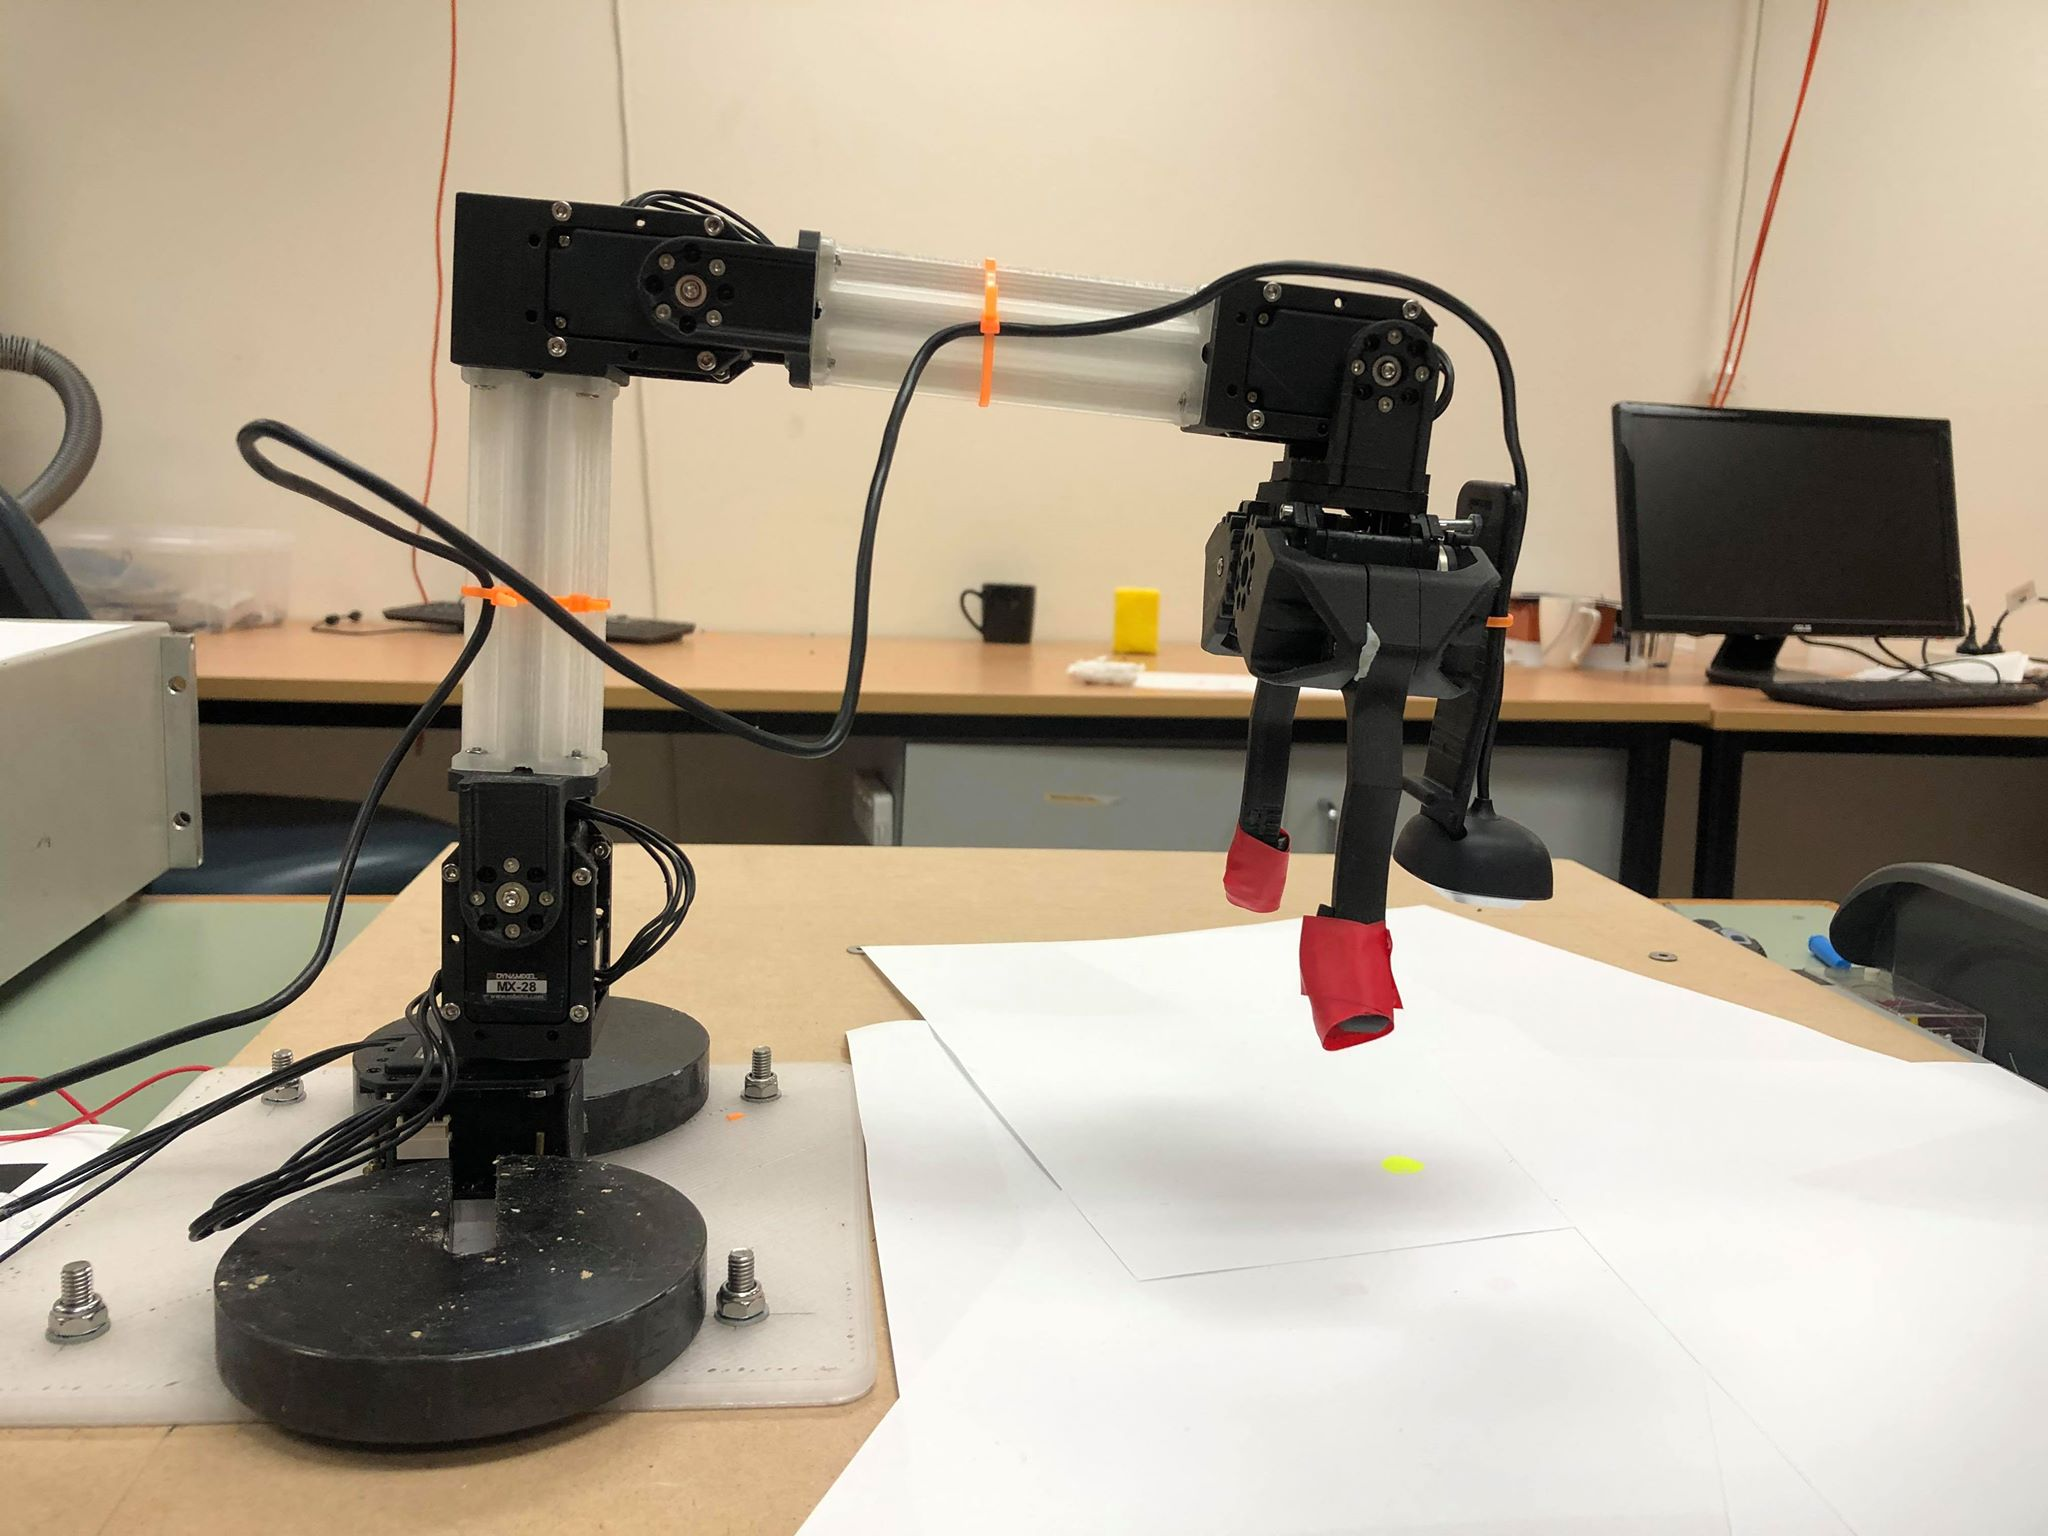
\includegraphics[width=.5\linewidth]{Figures/5DOFarm}
			\caption{5DOF desktop robot arm, pictured with MX-28 servos, 3D printed grasper (modified with rubber padding to increase grip) and mounted camera}
					\label{fig:5dofrobotarm}
		\end{center}
	\end{figure}
	
This arm comprised of 5 Robotis Dynamixel MX-28 servo actuators. Each motor has a serial interface that can be used to command and receive state information. An onboard PID controller is used to control motor-shaft angles and an encoder returns the current position. These motors were assembled using 3D printed parts and arranged as per Figure \ref{fig:5dofrobotarm}. 
	
The camera used for this project was a \textit{Microsoft HD-3000 LifeCam Webcam} and it's mounting to the robot is shown in Figure \ref{fig:Cameramounting}  . Other cameras were also considered but not implemented on the robot (Appendix \ref{App:Alternative Cameras}).\\

\begin{figure}[H]
	\begin{center}
		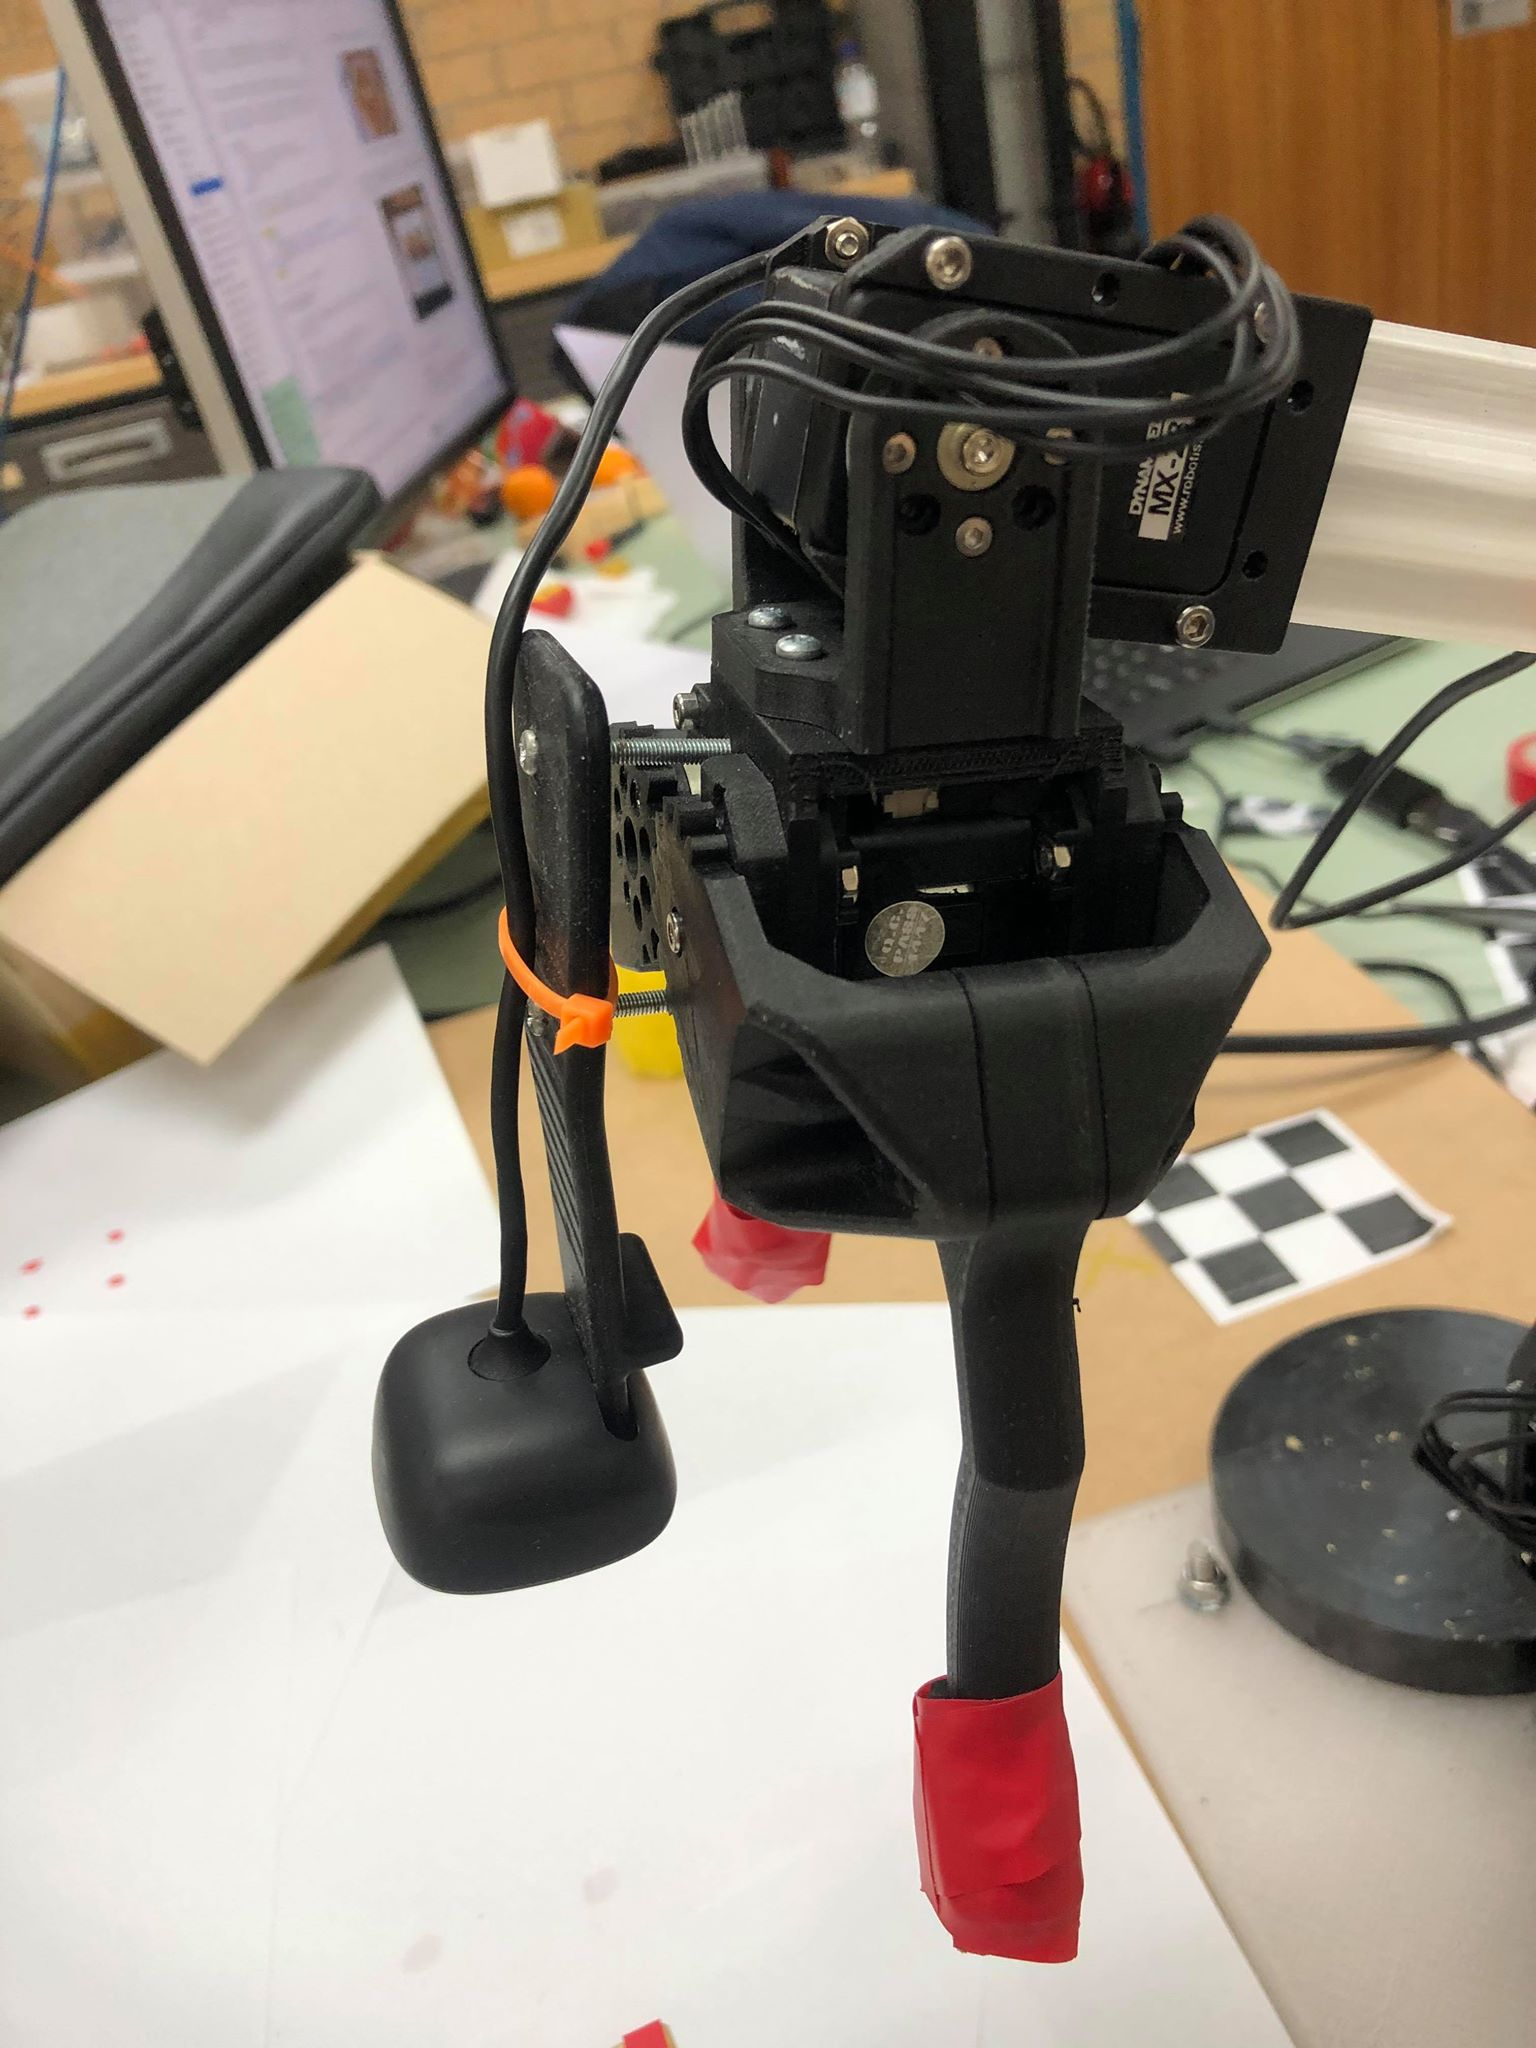
\includegraphics[width=.4\linewidth]{Figures/mountedCamera}
		\caption{The Microsoft camera mounted to the 5DOF robot arm}
		\label{fig:Cameramounting}
	\end{center}
\end{figure}	

The desired objects to be interacted with by the robot were a set of wooden blocks with animal figure cut-outs (Figure \ref{fig:PIGGYpic}). This common children's toy was chosen for it's uniform shape and the non-trivial classification problem it poses.

\begin{figure}[H]
	\begin{center}
		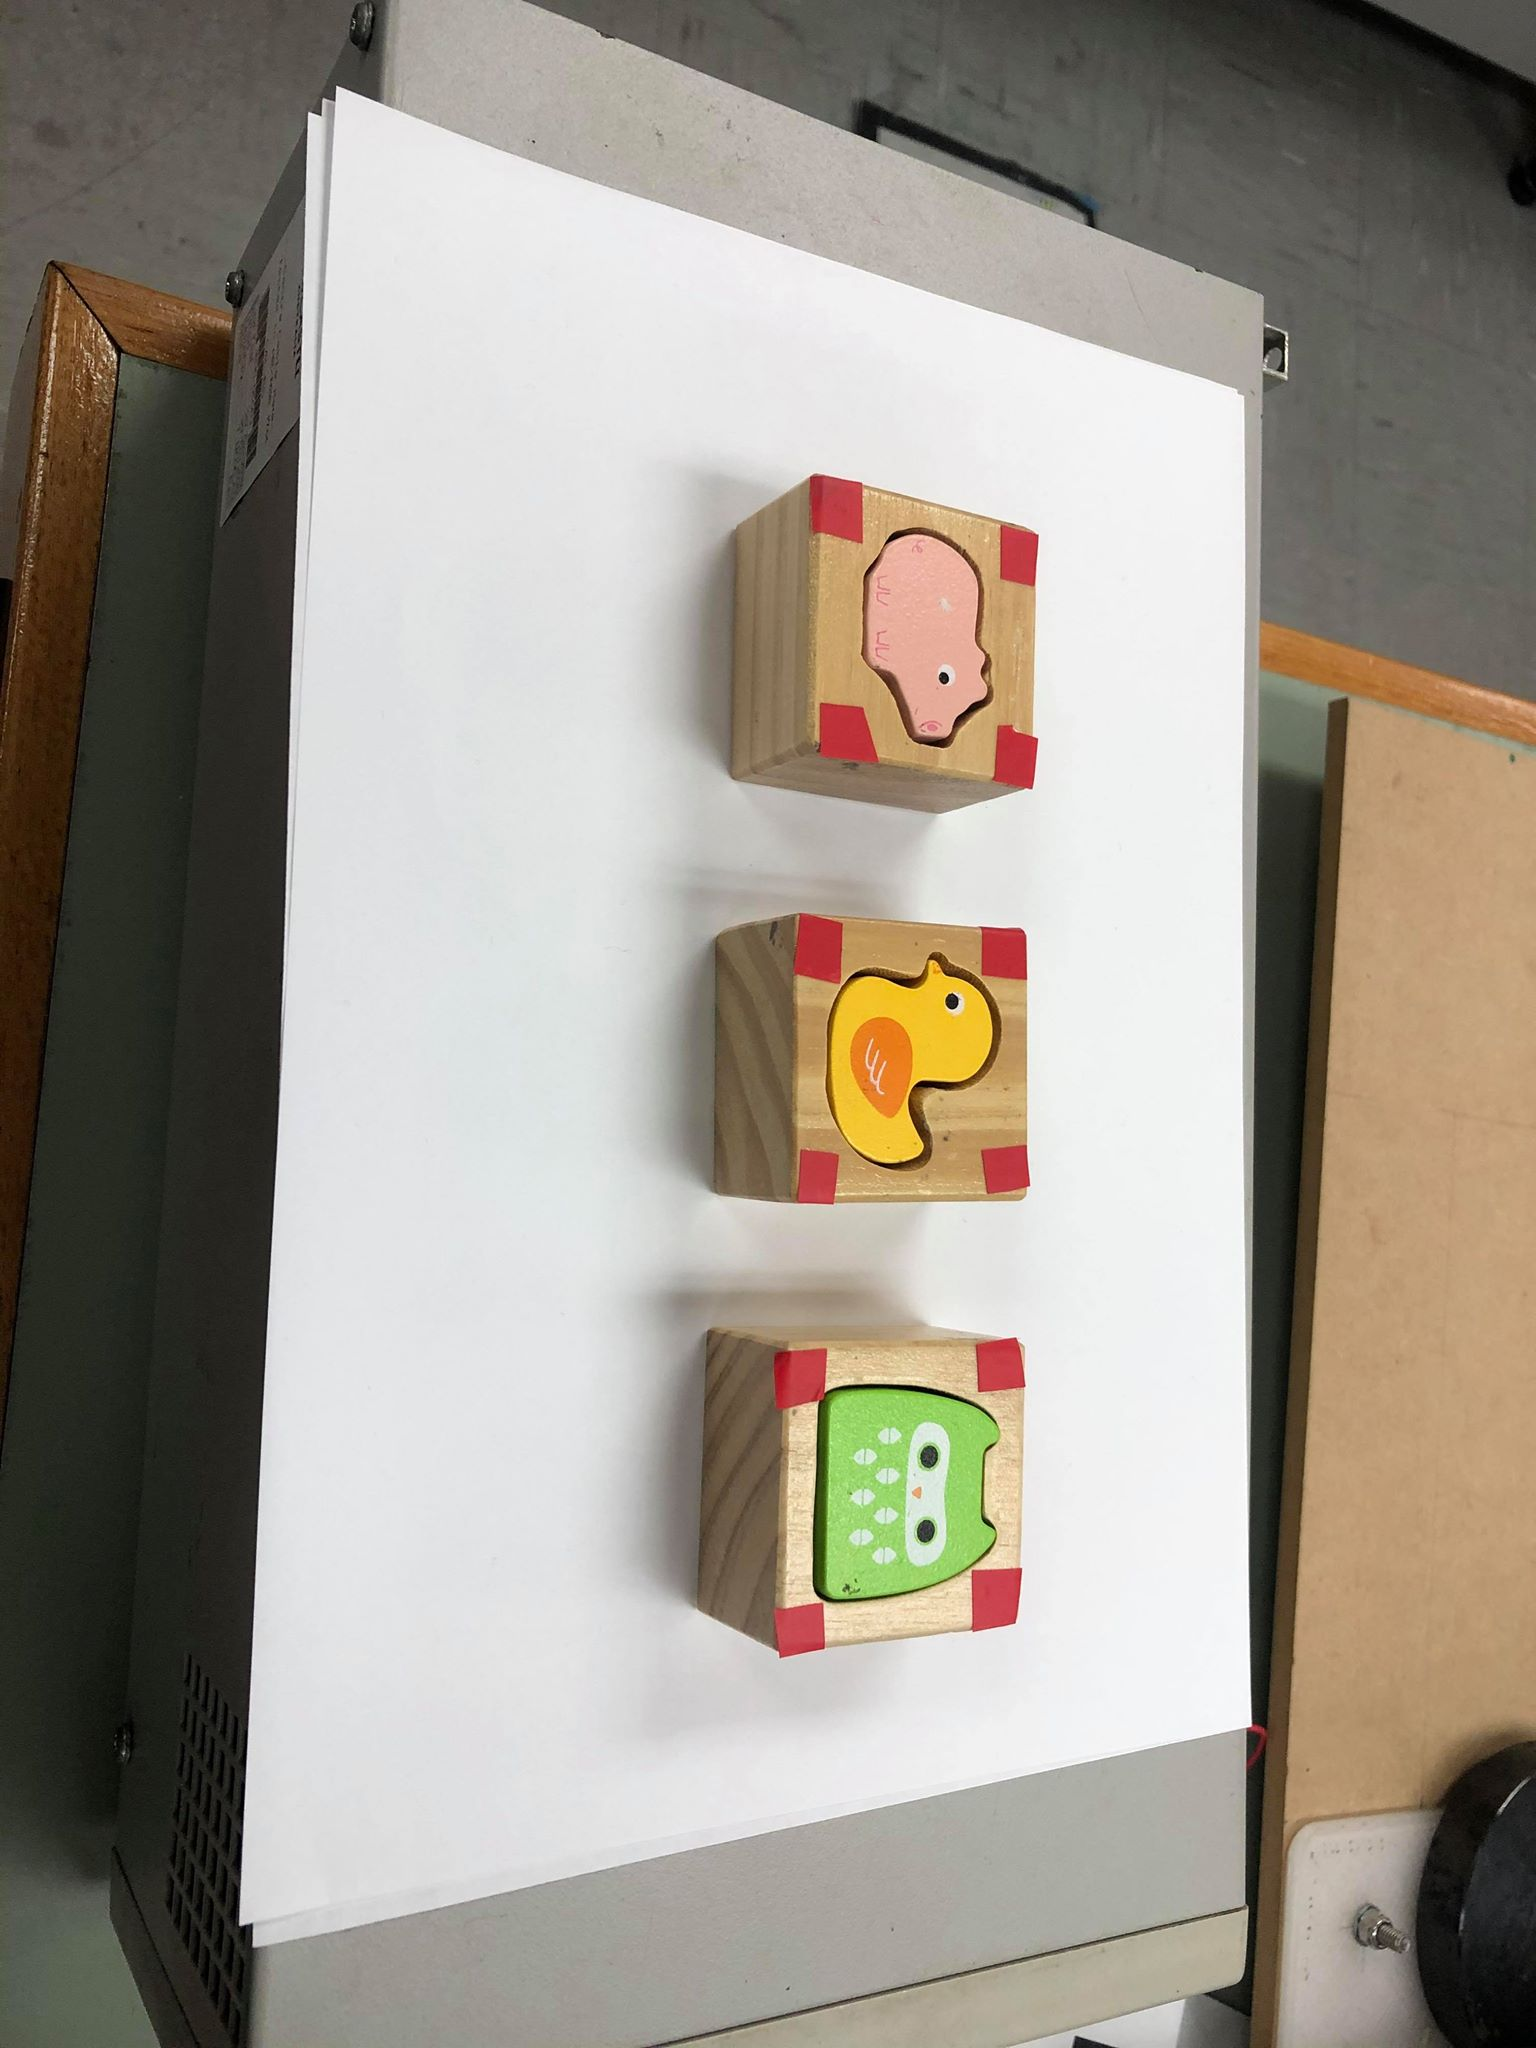
\includegraphics[width=.4\linewidth , angle = 90]{Figures/PIGGYpic}
		\caption{Wooden animal blocks used as the target object}
		\label{fig:PIGGYpic}
	\end{center}
\end{figure}

Finally, we can take a look at implementation.
	
%%%%%%%%%%%%%%%%%%%%%%%%%%%%%%%%%%%	
\subsection{Implementation}	

	Using the assumptions \ref{Assumptions}, \ref{Scope}, \ref{Literature Review} and considering the hardware available, the following implementation was proposed and forms the structure for the body of the report:
	
	\begin{itemize}
		\item Model and control the robot's motion using kinematics.
		\item Use a projection model to extract information from the camera.
		\item Train a neural-network-based object detector.
		\item Derive a visual servoing controller.
		\item Validate the prior points. Then integrate them to demonstrate a pick and place task.
	\end{itemize}
	

%%%%%%%%%%%%%%%%%%%%%%%%%%%%%%%
\newpage
\section{Robotic Manipulator Modelling}\label{sec:Core Section}

\begin{quote}
	''The mechanical structure of a robot manipulator consists of a sequence of rigid
	bodies(links)interconnected by means of articulations(joints);a manipulator is 
	characterized by an arm that ensures mobility,a wrist that confers dexterity, and an end 
	effector that performs the task required of the robot.'' \hfill \cite{siciliano2010robotics}
\end{quote}

Fundamentally, a robot arm is simply a series of actuated links that manipulate a end effector in a desired manner. To control a robotic manipulator, a suitable mathematical model is required that captures it's kinematics.\
This sections establishes the framework used to define motion and applies it to derive the kinematics of a robot. It then validates this approach in simulation and hardware.

%\subsection{ABB IRB 120}
%- introduce the robot and its specifications\\
%The IRB 120 is a 6DOF robotic manipulator commonly used in industry due to it's small size and high manuevarability. It can carry a payload of 3Kg at it's end effector, can reach 580mm horizontally from it's base and an end effector accuracy of 0.5mm. This makes it ideal for the desired pick and place task\\
%- The anthropomorphic structure of the ABB robot arm mimics the functionality of a real human arm, albeit with one less degree of freedom.\\
%- the desired end effector is not available and will be chosen or designed in part B. Such a system's design criterion and subsequent impacts with be further discussed in section XX\\
%- To use the robotic arm, a simulation model was required 
\subsection{Homogenous Transformation Matrix}\label{Homogenous Transformation Matrix}

\begin{figure}[H]
	\begin{center}
		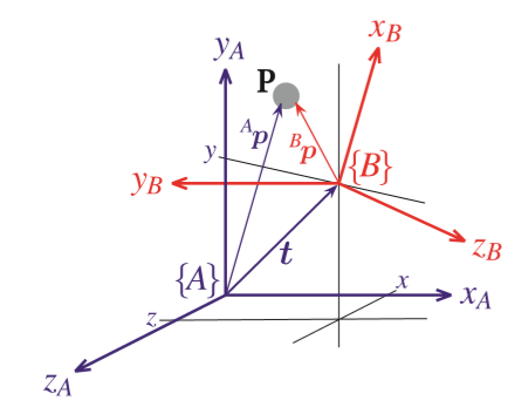
\includegraphics[width=.6\linewidth]{Figures/TransformationMatrix}
		\caption{A displacement and rotation from frame A to frame B}
		\label{fig:TransformationMatrix}
	\end{center}
\end{figure}

Whenever we describe the position or movement of an object, it is useful to have a point of reference from which the object is displaced. This point can be the origin of an orthogonal Cartesian co-ordinate system and any displacements can be described as a deviation from the origin along it’s x, y or z axis. This distance must be measured to a chosen point on the object, which will act as the origin of the objects own coordinate system. Thus, the displacement of object B can be referenced as its distance from object A as a  \textit{translation vector}. 

\begin{equation*}
\prescript{A}{}{\mathbf{t}}_{B} = \\
\begin{bmatrix}
X \\ Y \\ Z
\end{bmatrix}
\end{equation*} 

Similarly, rotations from one frame to the next can be described by an angular deviation about the principal axis. This can be represented by the \textit{rotation matrix}.

\begin{equation*}\label{eqn:rotationmatrix}
\prescript{A}{}{\mathbf{R}}_{B} = \\
\begin{bmatrix}
R11 & R12 & R13 \\
R21 & R22 & R23 \\
R31 & R32 & R33 \\
\end{bmatrix}
\end{equation*} 

Together, these describe the position and orientation of frame {A} with respect to frame {B}. This information can be succinctly written in a \textit{homogenous transformation matrix}.
 
\begin{equation*}
\prescript{A}{}{\mathbf{T}}_{B} = \\
\begin{bmatrix}
\prescript{A}{}{\mathbf{R}}_{B} & \prescript{A}{}{\mathbf{t}}_{B} \\
\mathbf{0}^{3 \times 1} & 1 
\end{bmatrix}
\end{equation*} 

where $\prescript{A}{}{\mathbf{T}}_{B}$ represents the homogeneous transformation matrix that transfroms a coordinate system $ \{a\} $ to align with a second space $\{b\}$. The pose $\mathbf{W} = [ X, Y , Z , \Omega_1 , \Omega_2, \Omega_3]^{\top}$ represents the location and orientation of point $B$. \\

Transformation matrices have some useful properties:

\begin{subequations}
	\begin{equation}\label{eqn:transformcommute}
		\prescript{A}{}{\mathbf{T}}_{P} = \prescript{A}{}{\mathbf{T}}_{B}\prescript{B}{}{\mathbf{T}}_{P}\\
	\end{equation}
	\begin{equation}\label{eqn:transforminvert}
			\prescript{A}{}{\mathbf{T}}_{B}^{-1} = \prescript{B}{}{\mathbf{T}}_{A}\\
	\end{equation}
\end{subequations}

Equation \ref{eqn:transformcommute} states that transformations commute. This allows us to determine the pose of $P$ with respect to $A$ given that we know the pose of B from A ($\prescript{A}{}{\mathbf{T}}_{B}$) and P from B ($\prescript{A}{}{\mathbf{T}}_{B}$).\\
Equation \ref{eqn:transforminvert} states that transformations are invertible. Knowing the pose of B from A can also be expressed as knowing the pose of A from B. \\

Thus, we have a powerful framework for describing how objects move using transformation matrixes. This will form the basis of our \textit{Kinematics}


%%%%%%%%%%%%%%%%%%%%%%%%%%%%%%%%%%
\subsection{Robotic Manipulator Kinematics}

A robotic manipulator can be seen as a sequence of rigid bodies, known as \textit{links}, interconnected by actuated \textit{joints}. This can be referred to as an \textit{open serial kinematic chain} and an example is shown in Figure \ref{fig:JointsRobotArm}. The frame $\{0\}$ acts as the \textit{base} of the chain and the goal of kinematics is to express the pose of all subsequent links with respect to the base. \\

\begin{figure}[hh]
	\begin{center}
		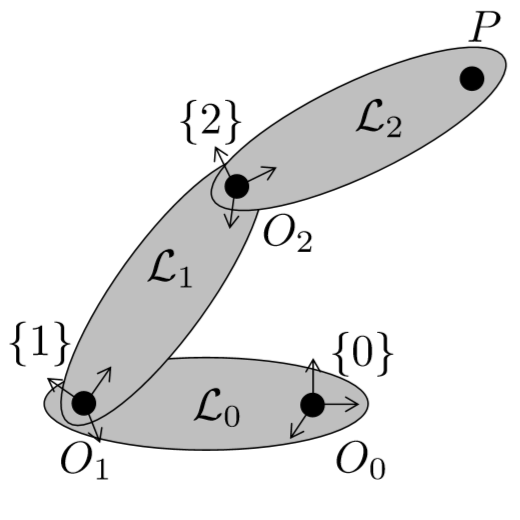
\includegraphics[scale=0.5]{Figures/JointsRobotArm}
		\caption{A serial kinematic chain, from \citep{RentonManipulatorDynamics}}
		\label{fig:JointsRobotArm}
	\end{center}
\end{figure}

This pose can be expressed through homogenous transformation matrixes (Section \ref{Homogenous Transformation Matrix}) by assigning a frame to each actuated joint. These joints are typically restricted to a single \textit{Degree of Freedom}: they can either rotate or extrude. These joints can be classified as $revolute$ or $prismatic$ joints respectively. \\

\newpage
%%%%%%%%%%%%%%%%%%%%%%%%%%%%%%%%%%
\subsubsection{Robotic Manipulator Forward Kinematics}

\begin{figure}[H]%
	
	\centering
	
	\subfloat[A 3D model of the arm with a gripper attachment in \cite{RoboDK}]{{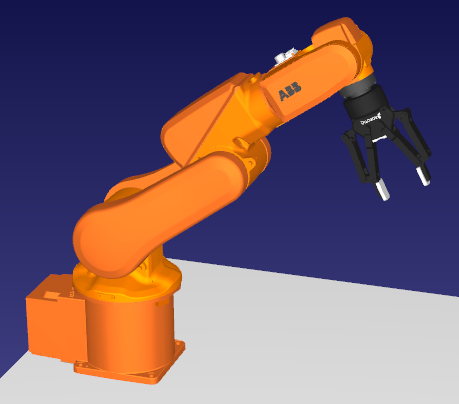
\includegraphics[scale=.6]{Figures/ABBrobotAnthroarm} }}%
	\hfil
	\subfloat[An anthropomorphic arm using revolute joints from \cite{siciliano2010robotics}]{{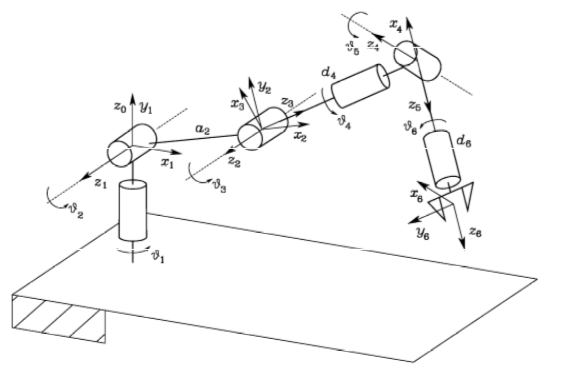
\includegraphics[scale=.7]{Figures/Anthroarm} }}%
	
	\caption{Modelling of the ABB IRB-120}%
	
	\label{fig:ABBrobotAnthro}%
	
\end{figure}

The ABB IRB-120 (Figure \ref{fig:ABBrobotAnthro}(a))is a 6DOF robotic manipulator, with 6 actuated joints in a \textit{anthropomorphic} configuration (Figure \ref{fig:ABBrobotAnthro}(b)). This arrangement is a form of biomimicry and imitates a biological arm with an \textit{elbow} and \textit{wrist}. The first, second and third joints form the elbow and control the \textit{position} of the subsequent joints while the fourth, fifth and sixth joints form the wrist and control the \textit{orientation} of the final frame. This final frame is known by convention as the \textit{end effector} and is located at the center of the gripper.\

The goal of Forward Kinematics is to obtain the pose of the last frame $x_e$, known as the end effector, with respect to the base frame. This can be expressed as:

\begin{equation}
	\prescript{0}{}{\mathbf{T}}_{e} = k(q)
\end{equation}

To do this we need to find the transformation matrices that relate the motion from each joint frame to the next as a function of joint angles $q$. We can then use the commutative property of transformation matrices \ref{eqn:transformcommute} to express this as:

\begin{equation}\label{eqn:Transformationmatrixjointangles}
	\prescript{0}{}{\mathbf{T}}_{e} = \prescript{0}{}{\mathbf{T}}_{1} \prescript{1}{}{\mathbf{T}}_{2} \prescript{2}{}{\mathbf{T}}_{3} \prescript{3}{}{\mathbf{T}}_{4} \prescript{4}{}{\mathbf{T}}_{5} \prescript{5}{}{\mathbf{T}}_{6} \prescript{6}{}{\mathbf{T}}_{e}
\end{equation}

Deriving these transformations from one joint to the next is not a straightforward task. Fortunately, 
the Denavit Hartenberg convention can be used. This convention is a methodology used to place and relate coordinate frames between joints and is used to generate the desired transformations \citep{hartenberg1964kinematic, hartenberg1955kinematic}.\\

As shown in Figure~\ref{fig:DH_photo} , it relates the coordinate frame between joint $j$ and joint $j+1$ using four parameters. The definition of each parameter is summarised in Table~\ref{tab:DHmeanings}/.

\begin{figure}[ht]
	\begin{center}
		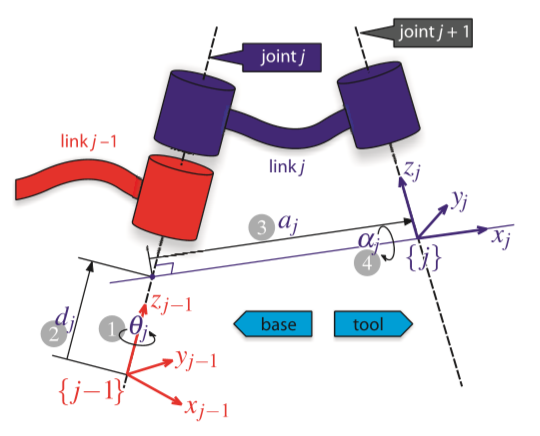
\includegraphics[width=.6\linewidth]{Figures/DH_photo}
		\caption{Transformation between two joints using the Denavit Hartenberg Convention, from Corke }
		\label{fig:DH_photo}
	\end{center}
\end{figure}

\begin{table}[H] 
	\caption{Denavit-Hartenberg parameters: their physical meaning, symbol and formal definition based on \cite{corke2017robotics}}
	\begin{tabular}{|l|l|l|l|}
		\hline
		Joint angle & $\theta$     & \begin{tabular}[c]{@{}l@{}}  The angle between the $ x_{j-1} $ and $ x_{j} $ \\  axes about the $ z_{j-1} $ axis  \end{tabular}                                & \begin{tabular}[c]{@{}l@{}}Variable for revolute joints;\\ Constant for Prismatic Joints\end{tabular} \\ \hline
		Link offset & d     & \begin{tabular}[c]{@{}l@{}}The distance from the origin of frame $ {j-1} $ \\  to the $ x{j} $ axis\end{tabular}                                            & \begin{tabular}[c]{@{}l@{}}Variable for Prismatic joints;\\ Constant for Revolute Joints\end{tabular} \\ \hline
		Link length & a     & \begin{tabular}[c]{@{}l@{}}The distance between the $ z_{j-1} $ and $ z_{j} $ axes along \\ the $ x_{j} $ axis; for intersecting axis parallel to \\ $  \hat{z}_{j-1} \times \hat{z}_{j} $ \end{tabular} & Constant for rigid links                                                                                              \\ \hline
		Link twist  & $\alpha$ &  \begin{tabular}[c]{@{}l@{}}The angle from the $ z_{j-1} $ axis to the $ z_{j} $ axis \\ about the $ x_{j} $ axis \end{tabular}                                                                                      & Constant for rigid links                                                                                             \\ \hline
	\end{tabular}
	\label{tab:DHmeanings}
\end{table}

Using this convention, transformations between joints can be expressed using the aforementioned parameters as 2 consecutive \textit{screw displacements} about the $z_j$ and $a_j$ axis. This can be expanded and rewritten as:

\begin{equation}
	\prescript{j-1}{}{\mathbf{T}}_{j} = \
	\begin{bmatrix}
		\cos{\theta_n} & -\sin{\theta_n} \cos{\alpha_j} & \sin{\theta_j} \cos{\alpha_j}  & r_j \cos{\theta_j} \\
		\sin{\theta_n} & \cos{\theta_n} \cos{\alpha_j}  & -\cos{\theta_j} \sin{\alpha_j} & r_j \sin{\theta_j} \\
		0           & \sin{\alpha_j}	 		  & \cos{\alpha_j}				& d_j\\
		0 			& 0						  & 0						& 1
	\end{bmatrix}
\end{equation}

which \textit{generates} transformation matrices as a function of 4 parameters. \

The Denavit hartenberg paramaters for the robot were found using \cite{RoboDKparams} and shown in Table \ref{tab:DHparamsABB}

\begin{table}[h]
	\centering
	\caption{Denavit Hartenberg parameters for ABB IRB 120}\label{tab:DHparamsABB}
	\begin{tabular}{l|llll}
		& \textbf{q} & \textbf{d} & \textbf{a} & $\mathbf{\alpha}$  \\ 
		\hline
		\textbf{Joint 1} & 0          & 0          & 290        & -pi/2           \\ 
		\hline
		\textbf{Joint 2} & -pi/2      & 270        & 0          & 0               \\ 
		\hline
		\textbf{Joint 3} & 0          & 70         & 0          & -pi/2           \\ 
		\hline
		\textbf{Joint 4} & 0          & 0          & 302        & pi/2            \\ 
		\hline
		\textbf{Joint 5} & pi/2       & 0          & 0          & -pi/2           \\ 
		\hline
		\textbf{Joint 6} & pi         & 0          & 72         & 0               \\
		\hline
	\end{tabular}
\end{table}\

Using the parameters from Table 1, the desired transformation matrices could be generated, 
with a fixed translation to get from the spherical wrist to the end effector.

Thus, we can now solve Equation \ref{eqn:Transformationmatrixjointangles}, which can be written in homogenous form:

\begin{equation}
\mathbf{\prescript{0}{}T_{ee}}=
\begin{bmatrix}
	\mathbf{\prescript{0}{}R_{ee}} &  \mathbf{\prescript{0}{}t_{ee}} \\
	\mathbf{0}      & \mathbf{1} 
\end{bmatrix}
\end{equation} 

and the pose can be more intuitively expressed using euler angles (see Appendix \ref{App:Euler Angles}) as:

\begin{equation}
\mathrm{\mathbf{x}}_e = 
\begin{bmatrix}
	x \\ y \\ z \\ \phi \\ \theta \\ \psi
\end{bmatrix}
\end{equation}

and the pose of the end effector is expressed as a function of joint angle \textit{q}:

\begin{equation}
	\mathrm{\mathbf{x}}_{e} = k(q)
\end{equation}

\subsubsection{Robotic Manipulator Inverse Kinematics}\label{Robotic Manipulator Inverse Kinematics}

Forward kinematics allows us map the joint angles $q$ in \textit{joint space} to the end effector pose $xe$ in \textit{Cartesian space}. As tasks are commonly prescribed in terms of position and orientation, we require a method to map a pose in Cartesian space to joint angles in \textit{joint space}. This mapping is known as a jacobian. This section borrows heavily from \cite{RentonDifferentialKinematics}. \

One method of solving the inverse kinematic problem numerically requires use of the \textit{geometric} and \textit{analytical} jacobians.\

The \textit{geometric Jacobian} relates the linear and angular velocity of the end effector in Cartesian space to the time derivative of joint angles in joint space and can be expressed as:

\begin{equation*}
	\mathbf{\nu}_e = \mathbf{J}_{G} (\mathbf{q}) \dot{\mathbf{q}}
\end{equation*}\

% = \mathbf{J_{v}}(q)\dot{q} \\
%\mathbf{\omega^{0}_{n}} = \mathbf{J_{\omega}}(q)\dot{q} 
where:
\begin{equation}
	\begin{aligned}
		\mathbf{\nu}_e  = 
		\begin{bmatrix}
			\mathrm{\mathbf{v}}^{0}_{e} \\ \mathbf{\omega}^{0}_{e}
		\end{bmatrix}
	\end{aligned}	
\end{equation}

The geometric jacobian can be generated for a series of revolute joints, using the notation given by the Denavit-Hartenberg convention, as:

\begin{equation}
	\mathbf{J} =
	\begin{bmatrix}
	\mathbf{J}_{v} \\ \mathbf{J}_{\omega}  
	\end{bmatrix} = 
	\begin{bmatrix}
	R^{0}_{j-1} \begin{pmatrix}
	0 \\0\\1 
	\end{pmatrix}(t^0_n - t^0_{j-1})\\
	 R^{0}_{j-1}
	 \begin{pmatrix}
	 0 \\0\\1 
	 \end{pmatrix}  
	\end{bmatrix}
\end{equation}\

Which is given for a 6DOF arm by:

\begin{equation*}
\mathbf{J} =
\begin{bmatrix}
J_{v_1} & J_{v_2} & J_{v_3} & J_{v_4} & J_{v_5} & J_{v_6}  \\
 J_{\omega_1} & J_{\omega_2} & J_{\omega_3} & J_{\omega_4} & J_{\omega_5} & J_{\omega_6}  
\end{bmatrix}
\end{equation*}\

Once again, we wish to prescribe the joint rates using a rate of change of euler angles. This can be done using the \textit{analytical jacobian}, which can be computed using:

\begin{equation*}
\mathbf{J_A} = \mathbf{T_A (R^0_n)J_G} 
\end{equation*}

where:

\begin{equation}
	\begin{aligned}
		\mathbf{T_A (R^0_n)} =
		\begin{bmatrix}
		\mathbf{I} & \mathbf{0} \\
		\mathbf{0} & \mathbf{E^{-1}(R^0_n)} 
		\end{bmatrix} 
	\end{aligned}
\end{equation}

and:
\begin{equation}
	\begin{aligned}
		\mathbf{E (R^0_n)} =
		\begin{bmatrix}
		1 & 0 & -\sin\theta\\
		0 & cos\phi & -\sin\phi cos\theta\\
		0 & -sin\phi & cos\phi cos\theta\\
		\end{bmatrix}
	\end{aligned}
\end{equation}

Thus, we have a direct relationship between the time derivative of the end effector pose $\mathrm{ \dot{\mathbf{x}}_e }$ and joint angles $\dot{\mathbf{q}}$ using the analytical jacobian:

\begin{equation} \label{eqn:AnalyticalJacobian}
	\mathrm{ \mathbf{\dot{x}}_e } = \mathbf{J_A \dot{q}}
\end{equation}

Given a desired pose:

\begin{equation}
\mathrm{\mathbf{x}}_d = 
\begin{bmatrix}
x \\ y \\ z \\ \phi \\ \theta \\ \psi
\end{bmatrix}
\end{equation} 

We can define an error:

\begin{equation*}
\mathbf{e} = \mathrm{ \mathbf{\dot{x}}_d } - \mathrm{ \mathbf{\dot{x}}_e }
\end{equation*}\

and take its time derivative as:

\begin{equation}
	\mathbf{\dot{e}} = \mathrm{ \mathbf{\dot{x}}_d } - \mathrm{ \mathbf{\dot{x}}_e } 
\end{equation}

into which we can substitute Equation \ref{eqn:AnalyticalJacobian} to give:

\begin{equation}\label{eqn:errorderivative}
	\mathbf{\dot{e}} = \mathrm{ \mathbf{\dot{x}}_d } - \mathbf{J_A(q) \dot{q}}
\end{equation}

If we consider the homogenous ordinary differential equation:

\begin{equation}
	\mathbf{\dot{e}} = \mathbf{K e}
\end{equation}

 we can rewrite Equation \ref{eqn:errorderivative} as:

\begin{equation} \label{eqn:inversejacobianequationIKM}
\mathbf{\dot{q}} = \mathbf{J_A(q)}^{-1} (\mathrm{ \mathbf{\dot{x}}_d } - \mathbf{K e})
\end{equation}

where $K$ is a diagonal matrix whose eigenvalues act as the \textit{gain} of a proportional controller. This is expressed as a block diagram in Figure \ref{fig:ode}. \\

\begin{figure}[H]
	\begin{center}
		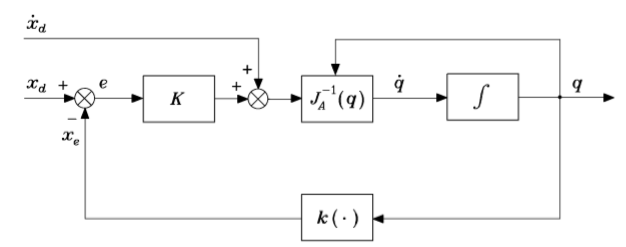
\includegraphics[width=.9\linewidth]{Figures/ode}
		\caption{Inverse kinematic model Control Scheme}
		\label{fig:ode}
	\end{center}
\end{figure}\

Provided that the analytical jacobian is square and of full rank and assuming a fixed reference ($\mathrm{ \mathbf{\dot{x}}_d }$), we can simulate equation \ref{eqn:inversejacobianequationIKM} to obtain a solution to our inverse kinematic problem.

Conversely, an optimisation based solution to the inverse kinematic problem can be implemented by posing problem as a nonlinear program: 

\begin{equation}
	\begin{aligned}
	\left(\mathbf{q}^{\star}, \mathbf{x}^{\star}\right)=& \arg \min _{\mathbf{q}, \mathbf{x}} \mathbf{q}^{\top} \mathbf{W} \mathbf{q}+\left(\mathbf{x}-\mathbf{x}_{e}\right)^{\top} \mathbf{K}\left(\mathbf{x}-\mathbf{x}_{e}\right) \\
	& \text { s.t. } \mathbf{x}-\mathbf{k}(\mathbf{q})=\mathbf{0}
	\end{aligned} 
\end{equation}

This can be solved using \texttt{fmincon}, a nonlinear programming solver in Matlab. This technique has the added benefit of allowing us to impose minimum and maximum joint angles as a lower bound( \texttt{lb}) and upper bound(\texttt{b}) respectively. \


%%%%%%%%%%%%%%%%%%%%%%%%%%%%%%%%%%%%%%%%%
\subsection{Simulation and Hardware}

The forward kinematic model for the ABB robot is shown as a "ball and stick" plot in Figure \ref{fig:fkmod}.

\begin{figure}[H]
	\begin{center}
		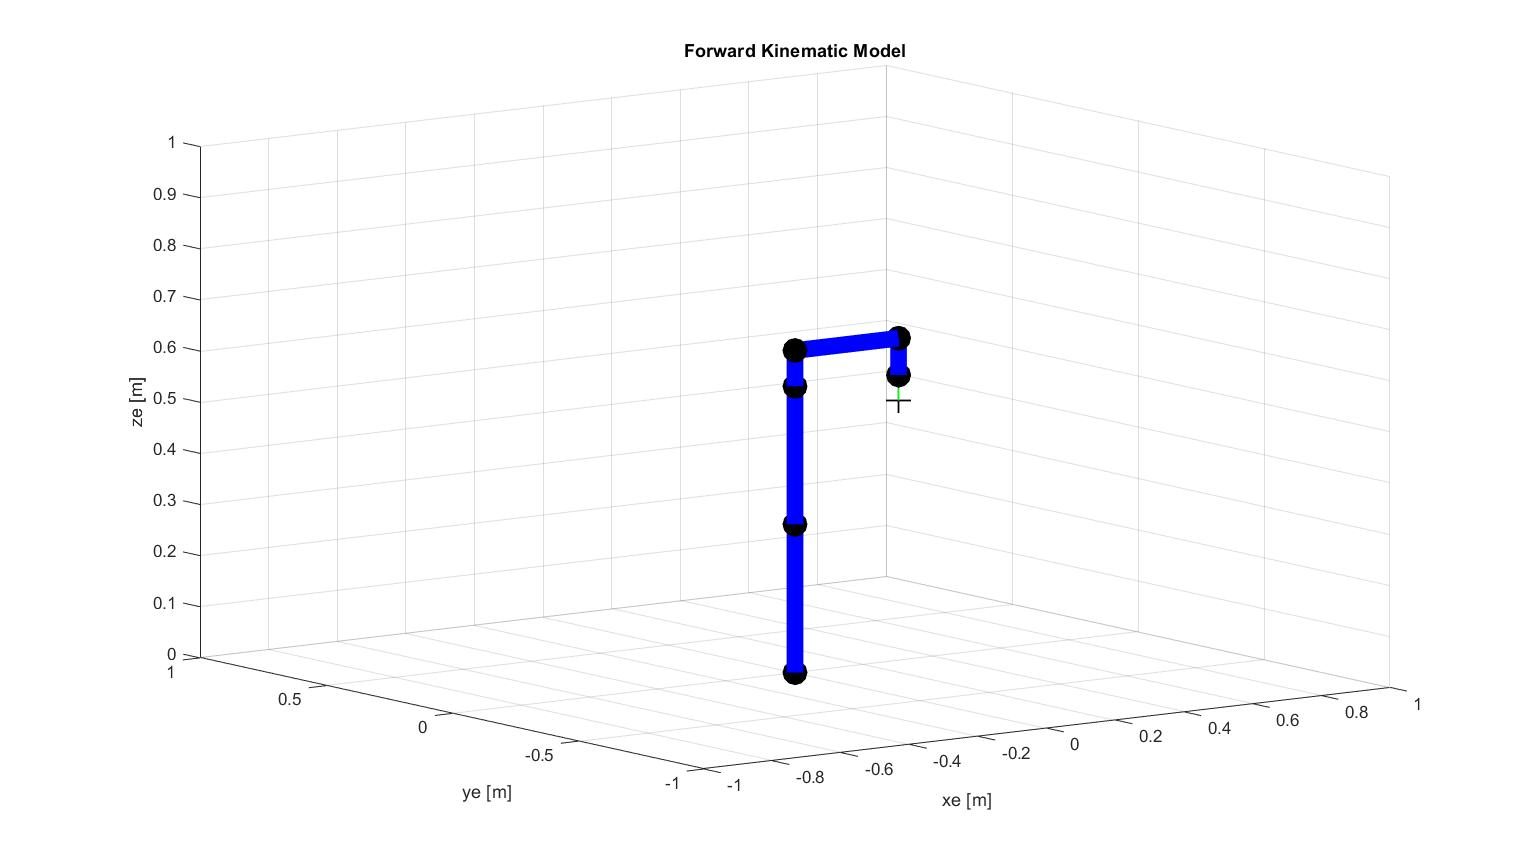
\includegraphics[width=.8\linewidth]{Figures/fkinmodel}
		\caption{Forward kinematic model simulation}
		\label{fig:fkmod}
	\end{center}
\end{figure}\

While it's inverse kinematics was used to follow a simple \textit{path} shown in Figure \ref{fig:ikmodel}.

\begin{figure}[H]
	\begin{center}
		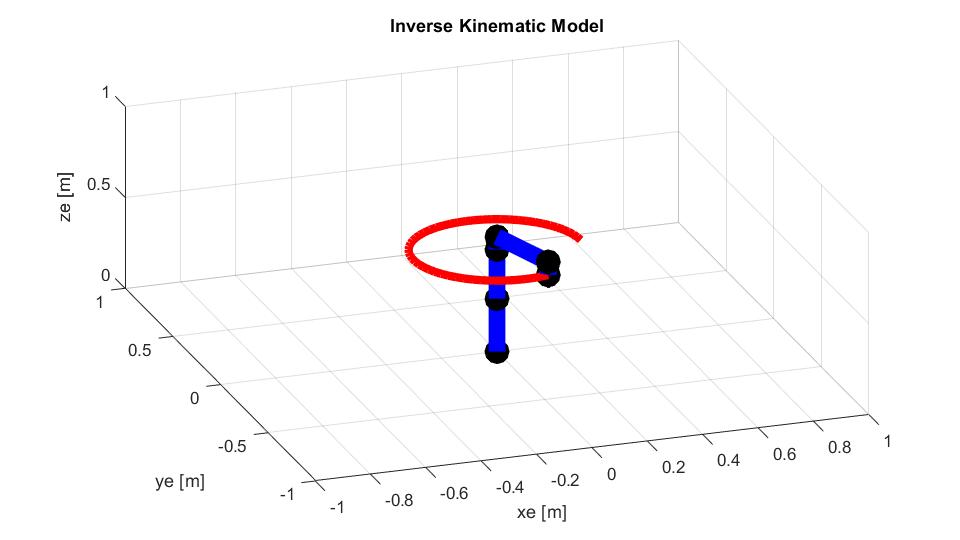
\includegraphics[width=.8\linewidth]{Figures/ikmodel}
		\caption{Inverse kinematic model Simulation}
		\label{fig:ikmodel}
	\end{center}
\end{figure}\

Due to issues accessing hardware highlighted in Section \ref{Hardware}, the forward and inverse kinematics were adapted for implementation with the 5DOF arm. Fortunately, this was relatively straightforward as the structure was largely the same. The actuators responsible for \textit{roll} and \textit{yaw} had their associated transformations set to \textit{\textbf{I}} and new values for the Denavit Hartenberg parameters were found. The new kinematic model is visualised in Figure \ref{FKMARM}.


\begin{figure}[H]
	\begin{center}
		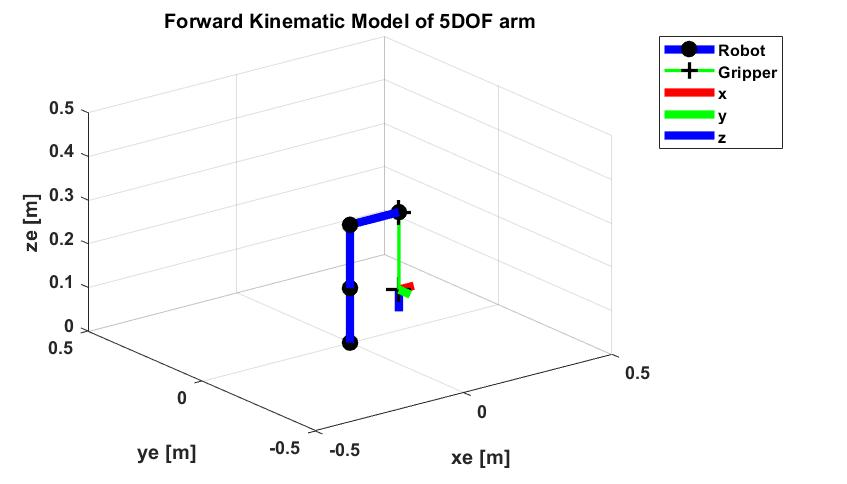
\includegraphics[width=.8\linewidth]{Figures/FKMARM}
		\caption{5DOF arm Forward kinematic model Simulation}
		\label{fig:FKMARM}
	\end{center}
\end{figure}\
  
It is important to note that only the first 4 joint angles $\mathbf{q}$ affect the pose of the robot while the final joint control the gripper. Additionally, the robot is no longer \textit{fully actuated} in its \textit{task space}. It can not independently achieve a prescribed roll or yaw angle and a desired pose can only be prescribed as:

\begin{equation}
\mathrm{\mathbf{x}}_d = 
\begin{bmatrix}
x \\ y \\ z \\ \theta \\
\end{bmatrix}
\end{equation} 



%%%%%%%%%%%%%%%%%%%%%%%%%%%%%%%%%%%%%%%
\newpage
\section{Camera Modelling}

Visual servoing relies on the relationship between real world points and how they are represented by cameras. This section defines the relationship using the camera projection model and subsequently introduces camera calibration, camera pose estimation and the Image Jacobian.

\subsection{Camera Projection Model}\label{Camera Projection Model}

Using a standard pinhole model, a camera projects a 3D world onto a 2D image plane as shown by Figure \ref{fig:CameraProjectionModel}.
 
\begin{figure}[H]
	\begin{center}
		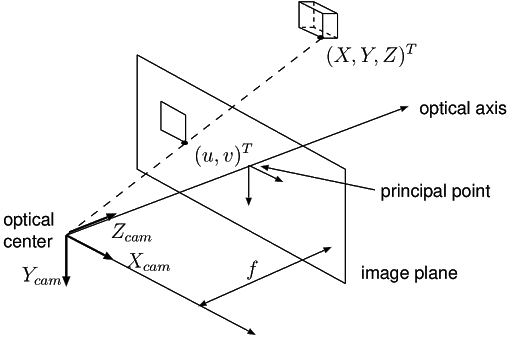
\includegraphics[width=.8\linewidth]{Figures/CameraProjectionModel}
		\caption{The Camera Projection Model}
		\label{fig:CameraProjectionModel}
	\end{center}
\end{figure}

\cite{zhang} describes this as the \textit{projection} of world point $P = [X Y Z]^{T}$ to the image point $p = [u v]^T$ through the function:

\begin{equation}\label{eqn:projectionequation}
p = \mathscr{P}(P,\mathbf{I},T_{cam})
\end{equation}

where $\mathbf{I}$ and $T_{cam}$ are the intrinsic and extrinsic parameters of the camera respectively. The extrinsic parameter is simply the pose of the camera, while its intrinsic parameters comprise of features such as the camera focal length ($f$), principal point ($u_0,v_0$) and camera skew ($\gamma$). This information is compiled into the \textit{Intrinsic Matrix}:

\begin{equation}
\mathbf{I} = \\
\begin{bmatrix}
f & \gamma & u_0 \\
0 & f & v_0 \\
0 & 0& 1
\end{bmatrix}
\end{equation} 

The projection model is based on an ideal projection through a pinhole whereas a real camera contains a non-ideal lens that distorts the image. Imperfect curvature of the lens manifests itself as radial distortion ( see Figure \ref{fig:RadialDistortion}).

\begin{figure}[H]
	\begin{center}
		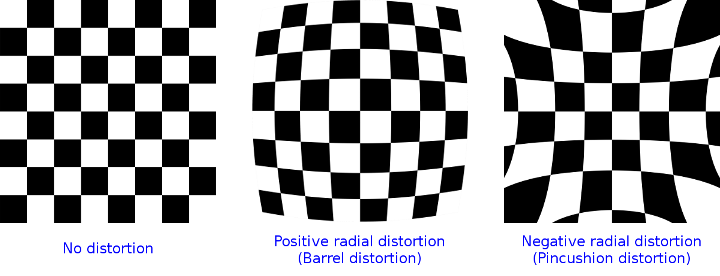
\includegraphics[width=.8\linewidth]{Figures/RadialDistortion}
		\caption{The effects of Radial Distortion}
		\label{fig:RadialDistortion}
	\end{center}
\end{figure}

whereas misalignment between the lens and image sensor causes tangential distortion (see Figure \ref{fig:TangentialDistortion}).

\begin{figure}[H]
	\begin{center}
		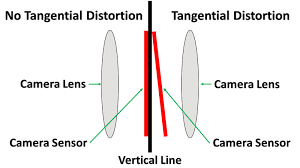
\includegraphics[width=.5\linewidth]{Figures/TangentialDistortion}
		\caption{The effects of Radial Distortion}
		\label{fig:TangentialDistortion}
	\end{center}
\end{figure}

These intrinsic parameters and distortions are unique to each camera and necessitate calibration. 

%%%%%%%%%%%%%%%%%%%%%%%%%%%%%
\subsection{Camera Calibration}\label{Camera Calibration}

Camera calibration is technique that estimates the intrinsic parameters and distortions of a camera \cite{zhang}. This estimation is done by  by exploiting the projection equation (\ref{eqn:projectionequation}).\

If the precise geometry of the world points and their projection at a variety of camera orientations is know, the intrinsic parameters of the camera can be estimated using a closed form solution and refined using maximum likelihood estimation. This refinement method can also be used to estimate the radial and tangential distortion of the camera.\

The calibration was performed using the Matlab Camera Calibrator toolbox \citep{bouguet2004camera}. This method involved collecting images of a planar checkerboard pattern (Figure \ref{fig:checkerboardpattern}) using the desired camera. 


\begin{figure}[H]
	\begin{center}
		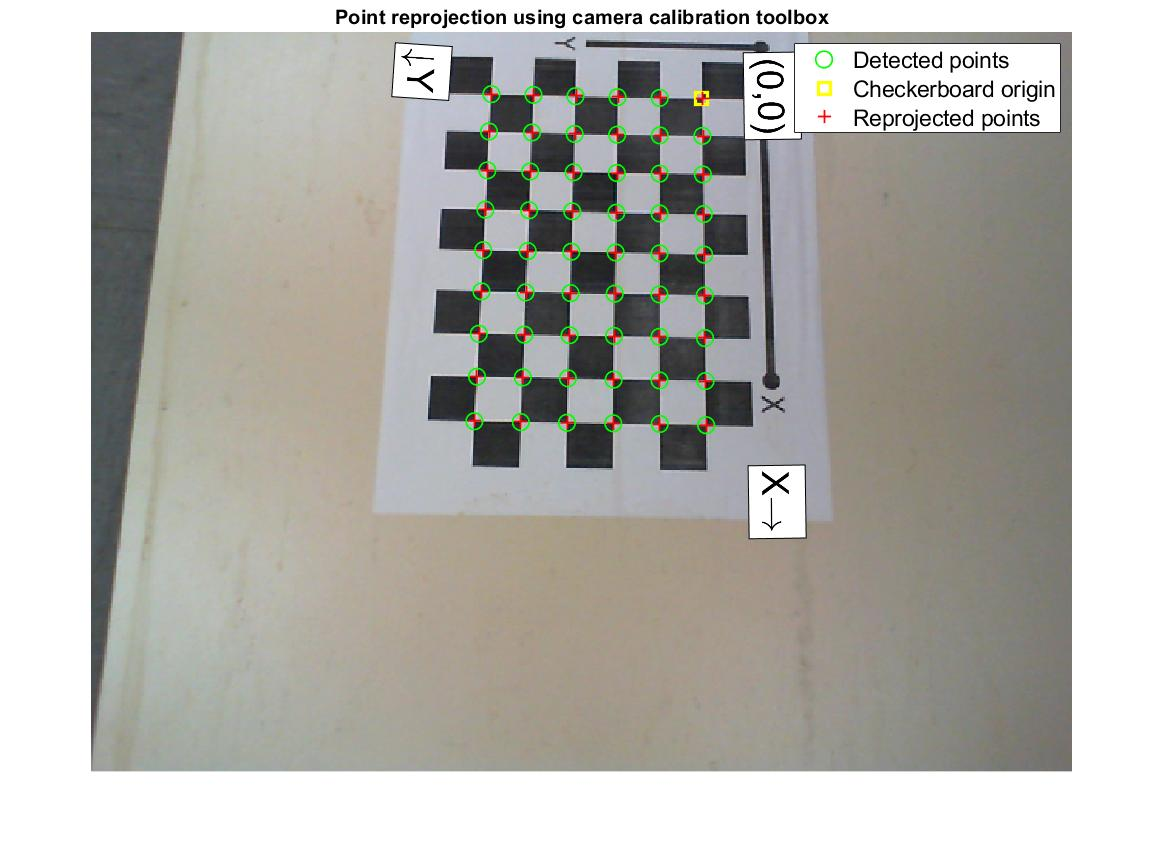
\includegraphics[width=.5\linewidth]{Figures/CalibrationImageExample}
		\caption{Checkerboard pattern with detected and re-projected feature points}
		\label{fig:checkerboardpattern}
	\end{center}
\end{figure}

The calibrator extracts the corners of the checkerboard as feature points (see Section \ref{Feature Point Extraction}) and then projects them to the image plane. By providing the toolbox with a precise measurement of the checkerboard squares, which are all identical, a precise geometric model can be formed.

\begin{figure}[H]%	
	\subfloat[Mean reprojection error in the calibration images ]{{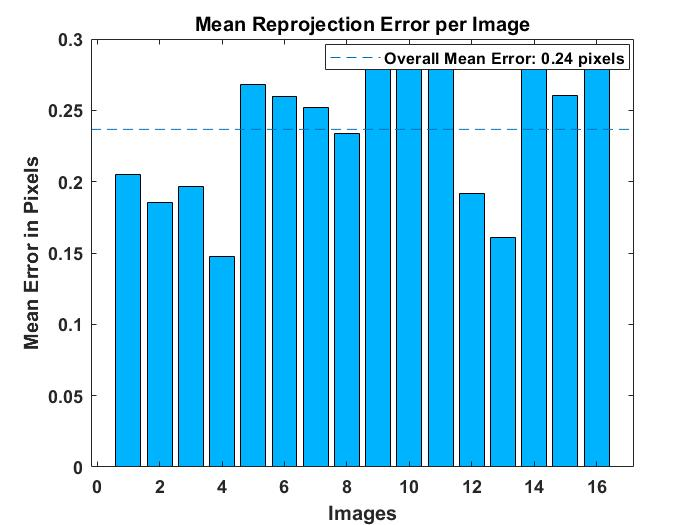
\includegraphics[scale=.35]{Figures/Reprojectionerror} }}%
	\
	\subfloat[Estimated relative pose between the camera and planar checkerboard]{{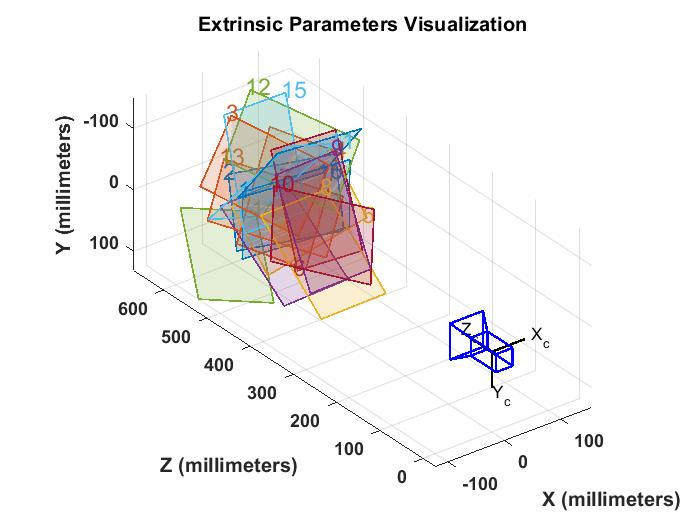
\includegraphics[scale=.35]{Figures/Extrinsicestimation} }}%
	
	\caption{Camera calibration results}%
	
	\label{fig:Im}%
	
\end{figure}


 The calibration procedure was then performed by the toolbox and the calculated parameters are shown in Table \ref{tab:CalculatedCameraParameters}.


\begin{table}[H]
	\caption{Camera Parameters for Microsoft HD-3000 LifeCam Webcam}\label{tab:CalculatedCameraParameters}
	\begin{center}
		\begin{tabular}{|c|c|c|}
			\hline
			Parameter 		        & Symbol    & Estimated Value                \\ \hline
			Focal length (mm)         & f         & 683.23               \\
			Principal point (pixels)      & $u_0,v_0$ & 322.1226 , 222.6395  \\
			Radial Distortion*     & $k_1,k_2$     & 0.2024 , -1.2111 \\
			Tangential Distortion* & $p_1 p_2$     & 0.0037 , 0.0019 \\
			Skew*				   & s         &     -1.4685    \\ \hline 
		\end{tabular}
	\end{center}
\hspace{3.5 cm} \vspace{0.25cm} * Unitless Parameter
\end{table}

%%%%%%%%%%%%%%%%%%%%%%%%%%%%%
\subsection{Feature Point Extraction}\label{Feature Point Extraction}

Our goal was to extract feature points from an image of the target objects shown in Figure \ref{fig:tagetobjectworkspace}


\begin{figure}[H]
	\begin{center}
		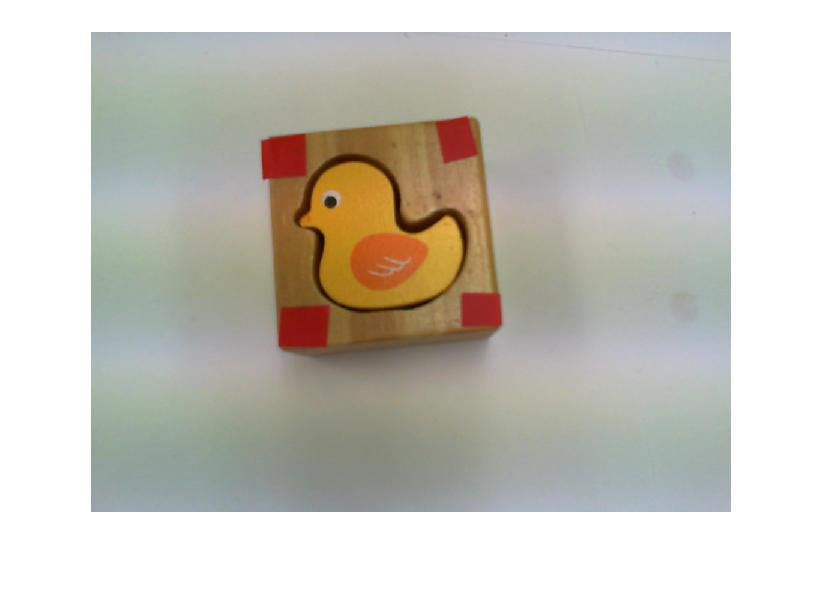
\includegraphics[width=.7\linewidth]{Figures/targetobjectworkspace}
		\caption{The target object with added tape}
		\label{fig:tagetobjectworkspace}
	\end{center}
\end{figure}



Objects are typically described by their characteristics such as size, shape and colour.
In images, measurements of these properties are known as \textit{features}. 
Techniques using corner and edge detection have been developed. However, it was difficult to reliably obtain corners due to shadows. Therefore, red tape was added to the corners to act as fiducials and colour thresholding was used. \

Images are digitally stored as an intensity in 3 RGB channels representing the red green and blue spectrum. 
We can simply extract the red channel and filter for a colour intensity corresponding to the tape that also minimises \textit{noise}.
This results in the image shown in figure \ref{fig:tagetobjectworkspacebw}, which consist of a set of interconnected pixels known as \textit{blobs}. 

\begin{figure}[H]
	\begin{center}
		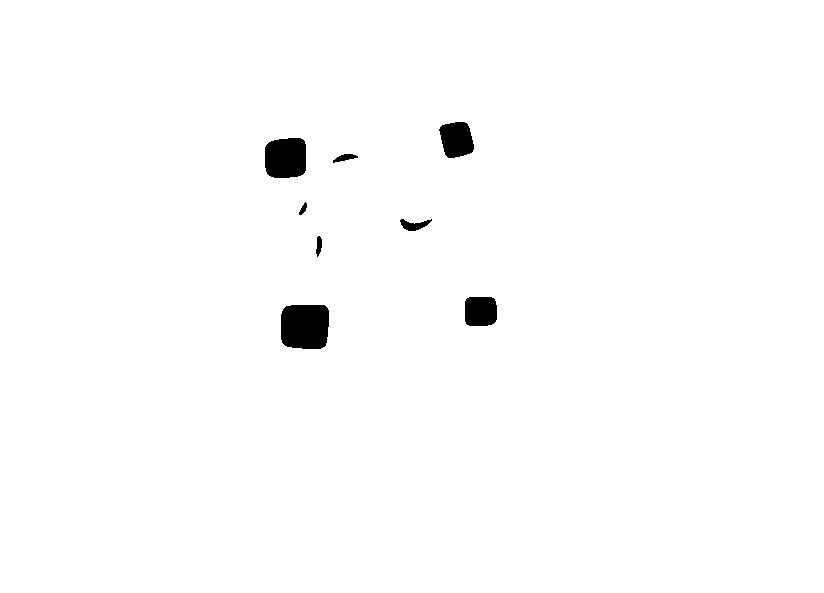
\includegraphics[width=.7\linewidth]{Figures/targetobjectworkspacebw}
		\caption{Figure \ref{fig:tagetobjectworkspace} after colour thresholding}
		\label{fig:tagetobjectworkspacebw}
	\end{center}
\end{figure}


We'd like to filter for the desired blobs corresponding to the tape and obtain the location of their centroid. This can be done using \textit{Region feature extraction}. 
An implementation of this method is available in the Machine vision toolbox by \cite{corke2017robotics} as a Matlab function called \texttt{iblobs}.

\begin{figure}[H]
	\begin{center}
		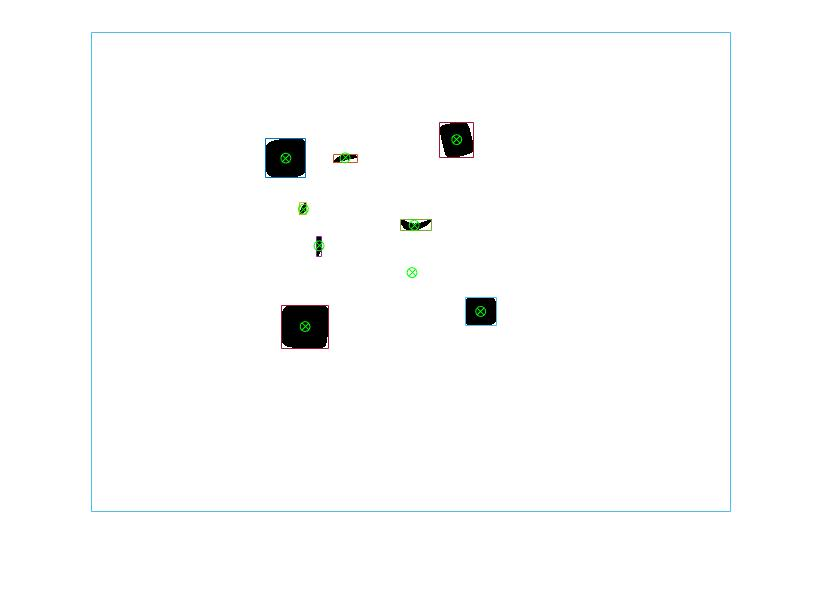
\includegraphics[width=.7\linewidth]{Figures/targetobjectworkspaceblobsall}
		\caption{The image after region feature extraction using \texttt{iblobs}}
		\label{fig:tagetobjectworkspaceblobsall}
	\end{center}
\end{figure}

Filtering for the desired blobs was done based on total \textit{pixel area} and \textit{aspect ratio}. Pixel area is simply a sum of a blob's pixels and values were chosen based on tuning.
The aspect ratio is based on transforming a blob into an equivalent ellipse (Figure \ref{fig:equivalentellipse}) with a major and minor axis length $a$ and $b$ respectively. This ratio is then defined as $\dfrac{b}{a}$ and can be used to indicate the \textit{circularity} of a shape. 
\begin{figure}[H]
	\begin{center}
		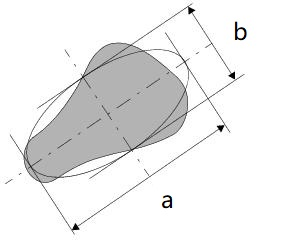
\includegraphics[width=.7\linewidth]{Figures/equivalentellipse}
		\caption{A blob and it's equivalent ellipse , retreived and modified from \citep{Microscan}}
		\label{fig:equivalentellipse}
	\end{center}
\end{figure}

The tape pieces were cut to a square shape to \textit{maximise} this circularity and allow robust filtering. Their \textit{centroid}, which is the average pixel coordinate of each pixel in a blob, was then extracted and used as our feature points. 
\begin{figure}[H]
	\begin{center}
		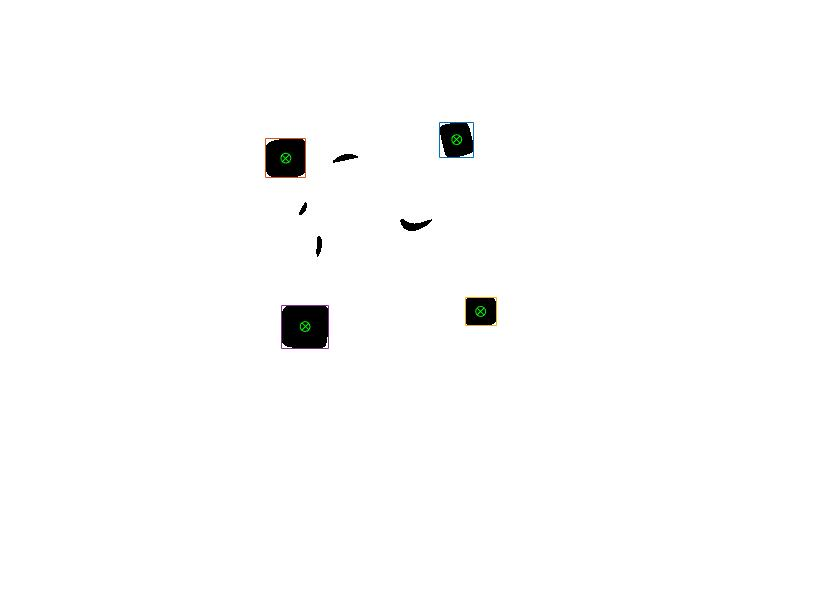
\includegraphics[width=.7\linewidth]{Figures/targetobjectworkspaceblobs}
		\caption{The desired feature points after filtering based on circularity}
		%		\label{}
	\end{center}
\end{figure}

The \textit{order} of these feature points was not guaranteed as they were sorted based on the raster order (smallest $v$ coordinate) of each blob. This order changes as the object or camera reorients itself and the feature points subsequently change coordinates. Therefore, the points were filtered by comparing  their current location to their previous and minimising the error. 

%%%%%%%%%%%%%%%%%%%%%%%%%%%%%
\subsection{Pose estimation}\label{Pose estimation}

Pose estimation was done using an implementation of \cite{ke2017efficient}. This functionality is implemented in the \textit{Machine Vision Toolbox} by \cite{corke2017robotics} as the \textit{Central camera class} method \texttt{estpose}.\ An example of a pose estimated by the camera using extracted feature points is shown in Figure \ref{fig:estimatedposevalidation}.

\begin{figure}[H]
	\begin{center}
		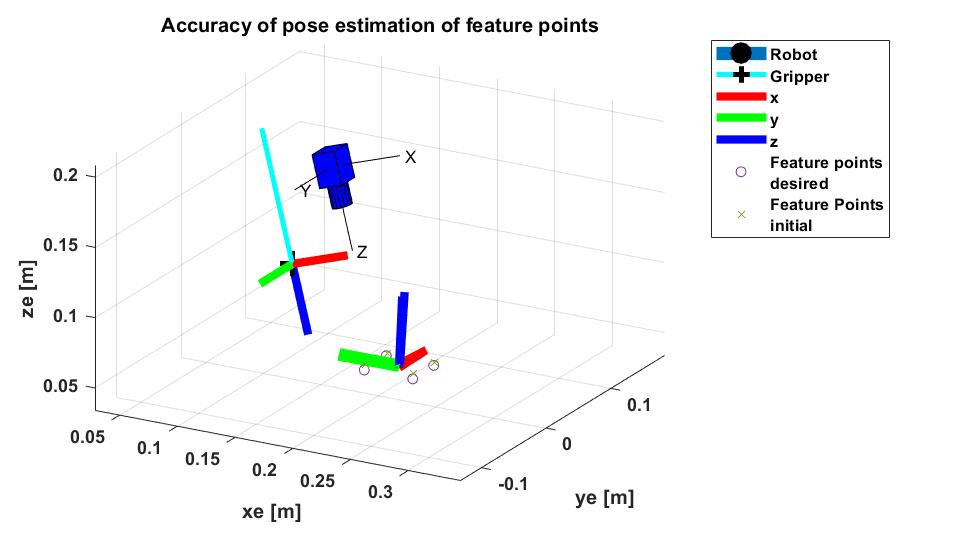
\includegraphics[width=.9\linewidth]{Figures/poseestimationvalidation}
		\caption{The estimated pose of the feature points at different camera orientations}
		\label{fig:estimatedposevalidation}
	\end{center}
\end{figure}

%%%%%%%%%%%%%%%%%%%%%%%%%%%%%
\subsection{Image Jacobian}\label{Image Jacobian}

Another useful relationship of the camera projection model is the \textit{Image Jacobian}, which relates the motion of world points to image points. This can be expressed as a derivative with respect to time of the projection equation \ref{eqn:projectionequation}: 


\begin{equation}
\dot{p} = \mathbf{J}_{P}(P,\mathbf{I},T_{cam})\mathbf{\nu}
\end{equation}

where $\dot{p}$ is the feature point velocity, $\nu$ the camera velocity and $\mathbf{J}_{P}$ is the Image Jacobian. If we consider point $\mathbf{P} = [X, Y, Z]^\top$ and camera with velocity $\mathbf{\nu} = [\mathbf{v} , \mathbf{\omega}]^{\top}$, the velocity of the points with respect to the camera frame is:

\begin{equation*}
\dot{\mathbf{P}} = \mathbf{-\omega \times  P - v}
\end{equation*}

which can be expressed in scalar form as:

\begin{equation} \label{eqn:ScalarForm}
\begin{aligned}
\dot{X} & = Y\omega_{z} - Z\omega_{y} - v_{x} \\
\dot{Y} & = Z\omega_{x} - X\omega_{y} - v_{y} \\
\dot{Z} & = X\omega_{y} - Y\omega_{y} - v_{z}
\end{aligned}
\end{equation}

The perspective projection of for normalized image plane coordinates is:

\begin{equation}
\begin{aligned}
x = \dfrac{X}{Z} & , & y = \dfrac{Y}{Z}
\end{aligned}
\end{equation}

Whose derivative with respect to time is, using the quotient rule:

\begin{equation}
\begin{aligned}
\dot{x} = \dfrac{\dot{X}Z -X\dot{Z}}{Z^2} ,& \dot{y} = \dfrac{\dot{Y}Z -Y\dot{Z}}{Z^2}
\end{aligned}
\end{equation}

Substituting in equation \ref{eqn:ScalarForm} and using $X = Zx, Y = Zy$ gives:

\begin{equation} \label{eqn:ScalarFormsubstituted}
\begin{aligned}
\dot{x} & = -\dfrac{1}{Z}v_{x} + \dfrac{X}{Z} v_{z} + xy\omega_{x} -(1+x^2)\omega_{y} + y\omega_{z} \\
\dot{y} & = -\dfrac{1}{Z}v_{y} + \dfrac{y}{Z} v_{z} + + (1+x^2)\omega_{x} - xy\omega_{y} - x\omega_{z}
\end{aligned}
\end{equation}

which can be written out in matrix form as:

\begin{equation} \label{eqn:pdottovelocity}
\begin{aligned}
\begin{bmatrix}
\dot{x} \\ \dot{y}  
\end{bmatrix}
& =
\begin{bmatrix}
-\dfrac{1}{Z} & 0 & \dfrac{X}{Z} & xy & -(1+x^2) & y \\
0 & -\dfrac{1}{Z} & \dfrac{y}{Z} & (1=y^2) & -xy & -x \\

\end{bmatrix}
\begin{bmatrix}
v_x \\ v_y \\ v_z \\ \omega_{x} \\ \omega_{y} \\ \omega_{z}
\end{bmatrix} 
\end{aligned}
\end{equation}

Thus, we have a relationship between camera spatial velocity and normalised image coordinate velocity. We now need to transform this \textit{image velocity} to \textit{pixel velocity}. The relationship between normalised image velocity and pixel coordinates is given by: 

\begin{equation}
	\begin{aligned}
		u = \dfrac{f}{\rho_{u}}x + u_{0} ,
		& u = \dfrac{f}{\rho_{v}}y + v_{0}
	\end{aligned}
\end{equation}

which can be rearranged to give:

\begin{equation}
	\begin{aligned}
		x = \dfrac{\rho_{u}}{f}\bar{u} ,
		& y = \dfrac{\rho_{v}}{f}\bar{v}
	\end{aligned}
\end{equation}

where $\bar{u} = u - u_0 , \bar{v} = v - v_0$ are the pixel coordinates relative to the principal point. The time derivative is:

\begin{equation}
	\begin{aligned}
		\dot{x} = \dfrac{\rho_{u}}{f}\dot{\bar{u}} ,
	  & \dot{y} = \dfrac{\rho_{v}}{f}\dot{\bar{v}}
	\end{aligned}
\end{equation}

This can be substituted into equation \ref{eqn:pdottovelocity}, giving:

\begin{equation}\label{eqn:ImageJacobiannormal}
\begin{aligned}
\begin{bmatrix}
	\dot{\bar{u}} \\
	\dot{\bar{v}}
\end{bmatrix}
& =
\begin{bmatrix}
-\frac{f}{\rho_{u} Z} & 0 & \frac{\bar{u}}{Z} & \frac{\rho_{v} \bar{u} \bar{v}}{f} & -\frac{f^{2}+\rho_{u}^{2} \bar{u}^{2}}{\rho_{u}f} & \frac{\rho_{v} \bar{v}}{\rho_{u}} \\

0 & -\frac{f}{\rho_{v} Z} & \frac{\bar{v}}{Z} & \frac{f^{2}+\rho_{v}^{2} \bar{v}^{2}}{\rho_{v} f} & -\frac{\rho_{u} \bar{u} \bar{v}}{f} & -\frac{\rho_{u} \bar{u}}{\rho_{v}}
\end{bmatrix}
&
\begin{bmatrix}
v_{x} \\
v_{y} \\
v_{z} \\
\omega_{x} \\
\omega_{y} \\
\omega_{z}
\end{bmatrix}
\end{aligned}
\end{equation}

As most image sensors use square pixels, we can assume $\rho_{u} = \rho_{v} = \rho $. This allows the focal length to be expressed in pixels as $f' = \dfrac{f}{\rho}$

\begin{equation}\label{eqn:ImageJacobian}
\begin{aligned}
\begin{bmatrix}
\dot{\bar{u}} \\
\dot{\bar{v}}
\end{bmatrix}
& =
\begin{bmatrix}
-\frac{f'}{Z} & 0 & \frac{\bar{u}}{Z} & \frac{\bar{u} \bar{v}}{f'} & -\frac{f'^{2}+ \bar{u}^{2}}{f'} & \bar{v} \\

0 & -\frac{f'}{Z} & \frac{\bar{v}}{Z} & \frac{f'^{2} + \bar{v}^{2}}{f'} & -\frac{\bar{u} \bar{v}}{f'} & -\bar{u}
\end{bmatrix}
&
\begin{bmatrix}
v_{x} \\
v_{y} \\
v_{z} \\
\omega_{x} \\
\omega_{y} \\
\omega_{z}
\end{bmatrix}
\end{aligned}
\end{equation}

Thus, we have our desired relationship between pixel motion with respect to the principal points and camera velocty. This can written as:

\begin{equation}
	\dot{p} = \mathbf{J}_{p} (\mathbf{p}\mathbf{Z})\nu
\end{equation}

Where $J_{p}$ is the image jacobian expressed as a function of point feature pixel coordinates $p$ and feature depth $Z$. \\
This equation can be vectorised for n feature points:

\begin{equation}\label{imagejacobianequationstacked}
	\begin{bmatrix} 
		u_{1}  \\
		v_{1}  \\
		u_{2}  \\
		v_{2}  \\
		\vdots \\
		u_{n}  \\
		v_{n}  \\  
	\end{bmatrix} = 
	{\begin{bmatrix} 
		J_{p}(p_{1} , Z_{1})   \\
		J_{p}(p_{2} , Z_{2})   \\
		\vdots \\
		J_{p}(p_{n} , Z_{n})
		\end{bmatrix}}\mathbf{\nu} 	
\end{equation} 

To ensure the Jacobian is full rank and nonsingular, a minimum of 3 feature points are required. 

%%%%%%%%%%%%%%%%%%%%%%%%%%%%%%%%%%%%%%
\newpage
\section{Object Detection}

Machine vision techniques such as \textit{nearest neighbor} or Support Vector Machines (SVM) can be used to \textit{classify} images \citep{li2009encyclopedia}. However, this technique requires image feature extraction if we wish to detect multiple objects in a single image.

A superior technique that has become increasingly popular since the success off ''Alexnet'' \citep{krizhevsky2012imagenet} is to use \textit{Convolutional Neural Networks} to perform classification. These have then been adapted to perform \textit{object detection}, the task of \textit{localising} and \textit{classifying} objects in an image.  The following discusses the \textit{intuition} behind convolutional neural networks and how one was trained.

\subsubsection{Background}
 
\cite{hubel1959receptive} performed experiments to investigate a cats visual system (Figure \ref{fig:catbrain}). By analysing the electrical signal produced by neurons in a cat's brain they were able to demonstrate the presence of ''specialised neurons that respond only to certain sensory information''.

\begin{figure}[H]
	\begin{center}
		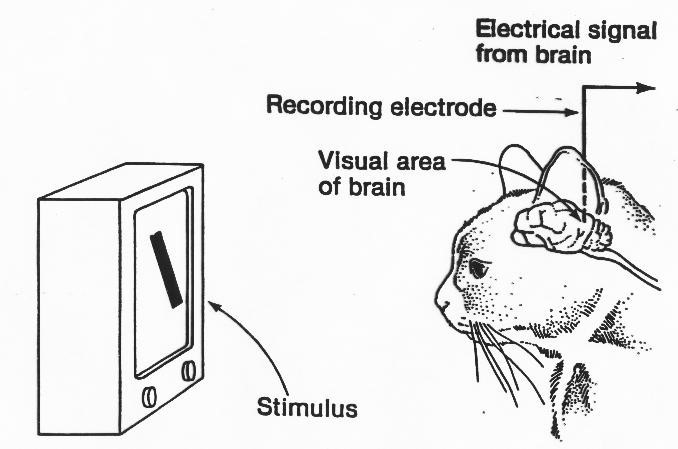
\includegraphics[width=.6\linewidth]{Figures/Catneuron}
		\caption{Experimental investigation of a cats visual system}
		\label{fig:catbrain}
	\end{center}
\end{figure}

Image features such as lines, curves and motion caused activity in different areas of neurons in the brain. This gave insight as to how a complex visual scene could be composed of simpler patterns that are detected by different groups of neurons.\
 

Artificial neurons have been modelled to mimic the functionality of biological neurons (Figure \ref{NEURONPERCEPTRON}.

\begin{figure}[H]
	\begin{center}
		\includegraphics[width=.7\linewidth]{Figures/Artificialneuron}
		\caption{A model of an artificial neuron}
		\label{NEURONPERCEPTRON}
	\end{center}
\end{figure}

which could be expressed by the equation:

\begin{equation}\label{eqn:Neuronequation} 
	y =  \psi 
	\begin{pmatrix} 
		\sum_{j=0}^{m} \omega\mathbf{x}
	\end{pmatrix}
\end{equation}

The cross product of the \textit{weights} and the \textit{inputs} results in a scalar value which is then outputed by a \textit{activation function }. If this activation function is chosen to be nonlinear, the output y is nonlinear. These individual nodes can then be stacked into a structure known as a \textit{neural network} (Figure \ref{fig:nnarch}) . \cite{252103} showed that various non-linear continious functions can be approximated using a neural networks with hidden layers. \

\begin{figure}[H]
	\begin{center}
		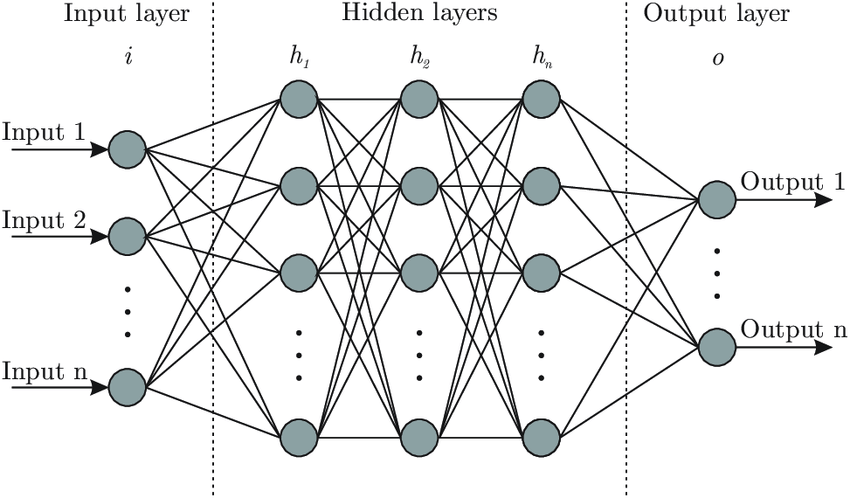
\includegraphics[width=.8\linewidth]{Figures/nnarchitecture}
		\caption{Basic architecture of a neural network, retrieved from \citep{neuralnetworkarch}  }
		\label{fig:nnarch}
	\end{center}
\end{figure}

This approximation is done by \textit{training} the network using \textit{backpropagation}. This technique uses a set of inputs that produce \textit{known outputs} $y^*$ for the function that needs to be approximated. Those same inputs are then computed through a suitable neural network producing a unique output $y$. If the weights of the neural networks are \textit{adjusted} such that $y^* - y$ is \textit{minimised}, the network tends towards an approximation of the desired function. 
These networks have been adapted to take in images as \textit{inputs} and approximate the nonlinear function of object classification and location.

%%%%%%%%%%%%%%%%%%%%%%%%%%%%%%%%%
\subsubsection{Training and Validation}

For the case where multiple objects might be in an image, we'd like to not only classify the object but also know where in the image it is. This can be accomplished using a Faster Region-based convolutional neural network (Faster RCNN). A Faster RCNN was selected based on the performance criteria available at the tensorflow github repository \cite{github}. This was because it was very accurate at the cost of being slower than other architectures such as YOLO or SSD.
Fortunately, a Faster RCNN model does not need to be designed from scratch as models are already available on Tensorflow, which provides a framework for designing and training neural networks. These models are pretrained on large datasets that allows them to detect common everyday objects. Using a pretrained model and adapting it for a new classifcation task is called \textit{transfer learning}. This technique \textit{hotstarts} the training process and greatly reduces the computational time required to perform reliable object detection.
Training to detect the target objects mention in Section \ref{Hardware} required generating a custom dataset. Research suggested a minimum of 100 images of each \textit{class} be used for successful detection. It was later found after training that extending this dataset to 250 images of each class provided a much more robust detector. Examples of the images used for training are shown in Figure \ref{fig:dataset}.  
Dataset generation also required labelling each image. This was done using an open-source labelling tool called \textit{Labelmg}.

\begin{figure}[H]
	\begin{center}
		\centering
		
		\subfloat[Example of varying lighting conditions]{{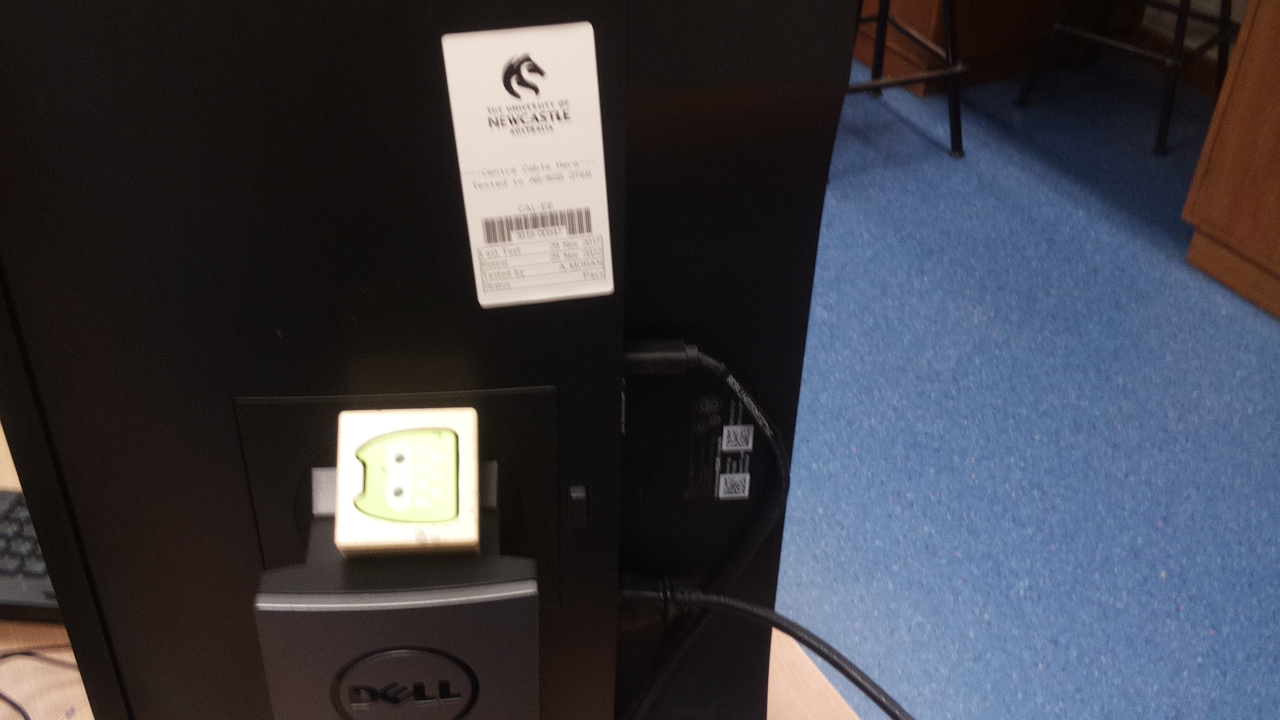
\includegraphics[scale=.2]{Figures/varyinglight} }}%
		\hfil
		\subfloat[Example of an occluded image]{{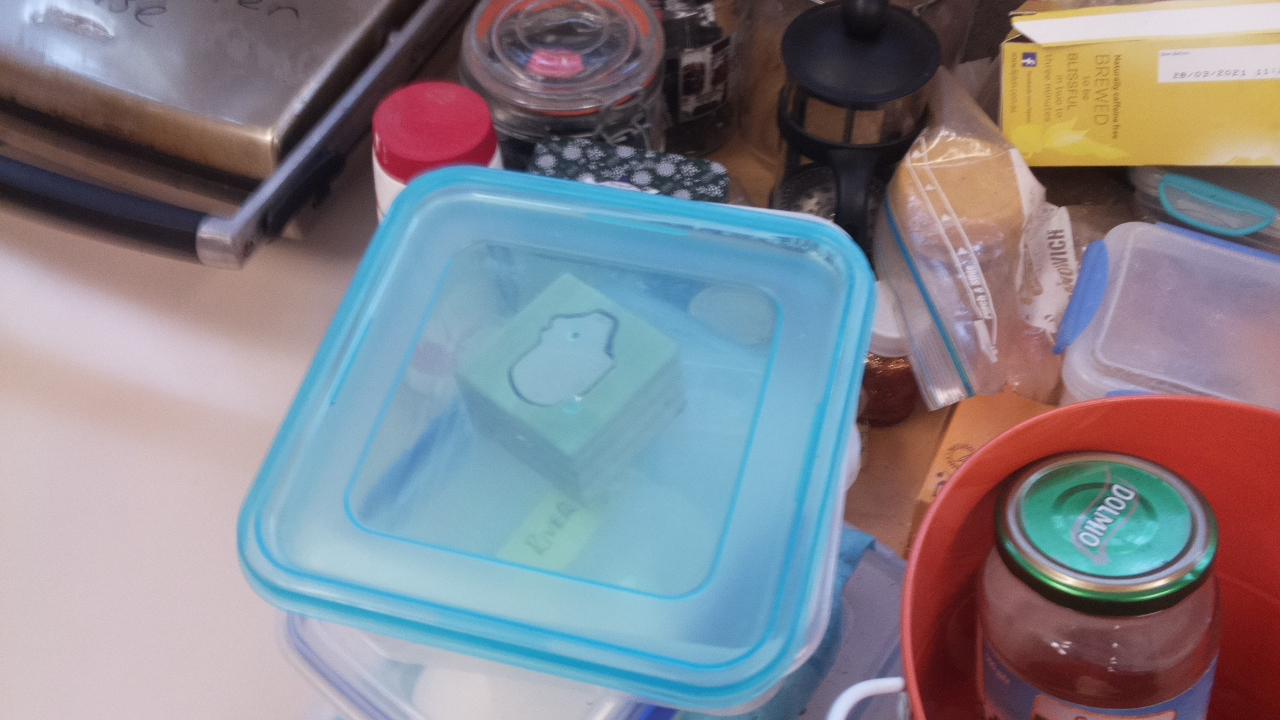
\includegraphics[scale=.2]{Figures/occlusion} }}%
	
		\subfloat[Example of captured image]{{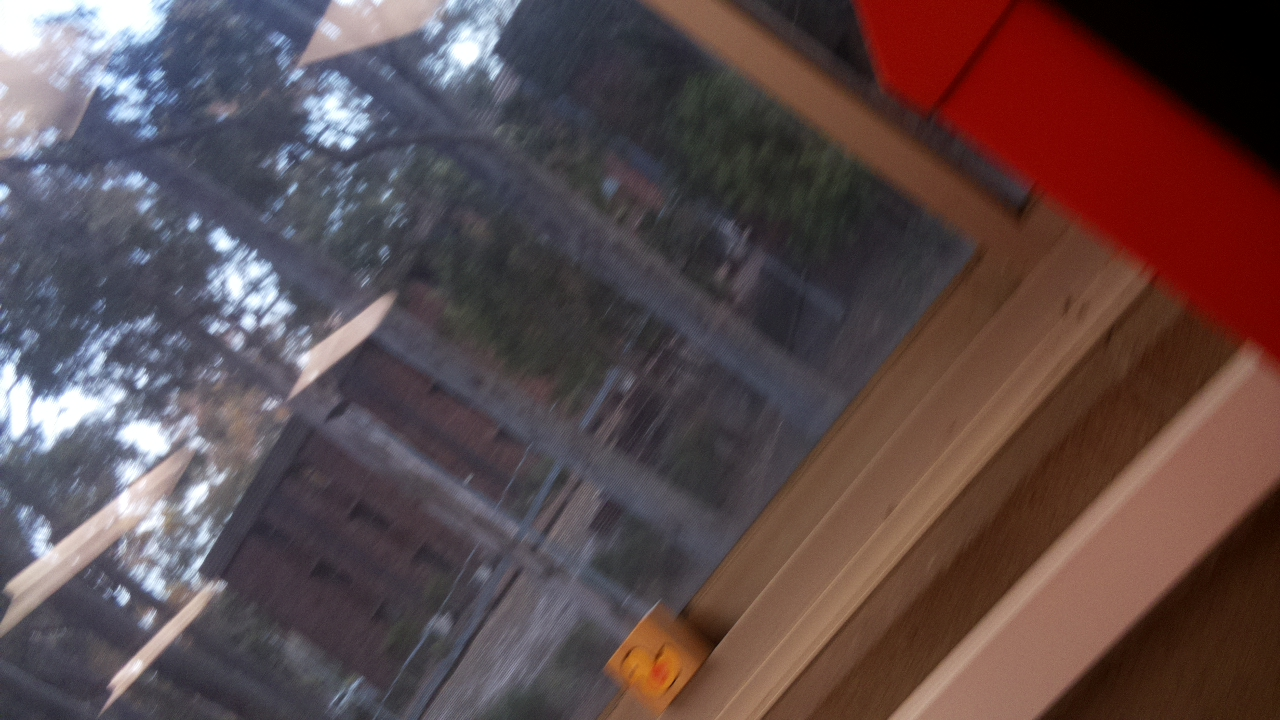
\includegraphics[scale=.2]{Figures/noisybackground} }}%
					
		\caption{Example of noisy backgrounds}%
		\label{fig:dataset}%
	\end{center}
\end{figure}

Large variations of the dataset prevents \textit{overfitting}, where variation or sample size is too low and the model starts learning to predict the dataset rather than the generalising. 
Variation included varying light saturation and intensity, noisy backgrounds and partial occlusions of the target object.

Additionally, before training additional \textit{preprocessing} was performed to inflate the dataset. This included randomly converting images to black and white, random rotations of the image and random saturation changes. 

This model was trained and Figure \ref{tensorboard} shows the \textit{loss} over training steps. 

\begin{figure}[H]
	\begin{center}
		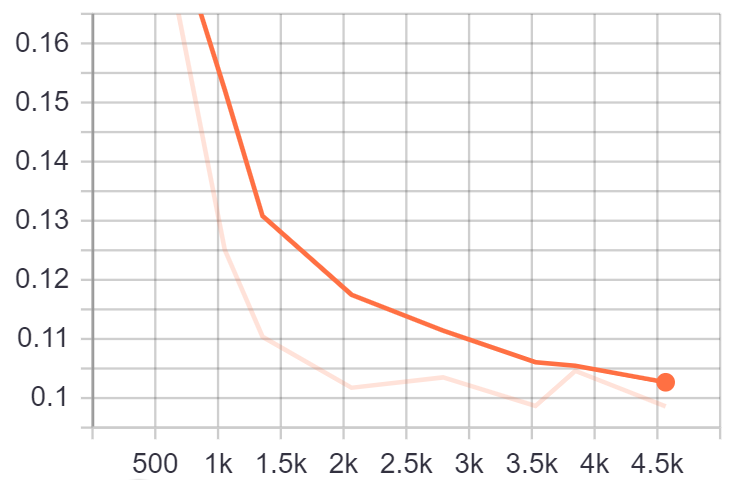
\includegraphics[width=.6\linewidth]{Figures/tensorboard}
		\caption{The loss over time as the model trained}
		\label{tensorboard}
	\end{center}
\end{figure}

The resultant object detector can be seen successfully detecting the desired objects with high accuracy in Figure \ref{detection}. It was proven to be robust and performed well under natural lighting conditions and partial occlusions.

\begin{figure}[H]
	\begin{center}
		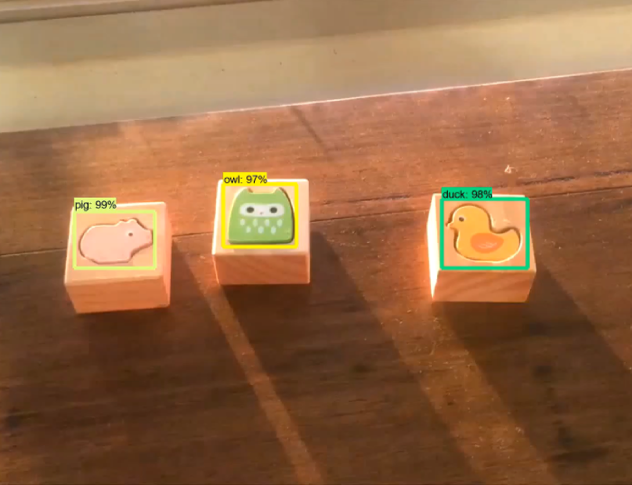
\includegraphics[width=.6\linewidth]{Figures/detection}
		\caption{Successful detection of target objects}
		\label{detection}
	\end{center}
\end{figure}

%%%%%%%%%%%%%%%%%%%%%%%%%%%%%%%%%%%%%%%%%
\newpage
\section{Visual Servoing}

Visual servoing aims to mimic the natural skill of hand-eye coordination. Instead of a robot operating in a fixed environment where the location of all objects is known, the robot is now able to operate in dynamic environments. This is facilitated by a visual sensor, which allows a vision-based feedback loop. Now a robot can observe the target object and interact with it without any prior indication of its pose. 
This approach requires continuous measurement of the targets and controls the robot accordingly, which allows for any errors in the system to be corrected over time.

This can be done using either a camera rigidly attached to the end effector of the robot, as shown in Figure \ref{fig:eyeinhandvseyeinsky} in an \textit{eye-in-hand} configuration. It could also be done using a fixed camera which overlooks the workspace in an \textit{eye-to-hand} configuration shown in the same figure. There are also hybrid approaches, which combine information from multiple cameras in either or both configurations \citep{tsai2014hybrid}. \

As specified by the Objective \ref{Objective}, the eye-in-hand configuration must be used and will subsequently be explored in this section.

\begin{figure}[H]
	\begin{center}
		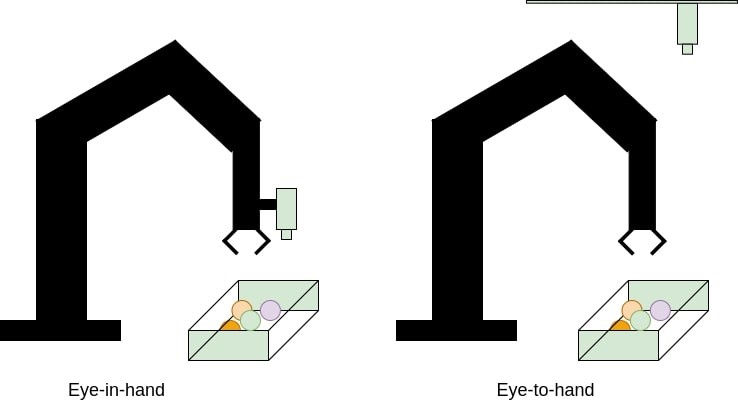
\includegraphics[width=.6\linewidth]{Figures/eyeinhandvseyeinsky}
		\caption{The 2 classes of visual servoing}
		\label{fig:eyeinhandvseyeinsky}
	\end{center}
\end{figure}

Additionally, There are various choices of camera that can be used, such as stereo cameras, fish-eye lens cameras and LIDAR units. These can all influence the type and amount of data that is collected. For this project, only a \textit{monocular} camera with a standard lens was considered based on the hardware available.

There are two fundamental approaches to visual servoing. There is position based visual servoing, which extracts feature points from an image, estimates the pose of the target object using those feature points and then performs a control action using the estimated pose. This task takes information from the image space and projects it to the cartesian space to perform control. This differs fundamentally from image based visual servoing, which extracts features from the image and then performs a control action entirely in the image space. There are also hybrid approaches which combine the two methods.  

The following subsections will discuss these various approaches.


\subsection{Position Based Visual Servoing }\label{PBVS}

Position Based Visual Servoing(PBVS) relies on estimating the pose of an object relative to the camera, then using this information to move to a desired pose relative to the object. This approach requires knowledge of the cameras intrinsic parameters , pose estimation , a joint controller for the robot, feature extraction and a model of the target objects geometry. The control scheme is shown in Figure \ref{fig:PBVScontrolscheme}. 

\begin{figure}[H]
	\begin{center}
		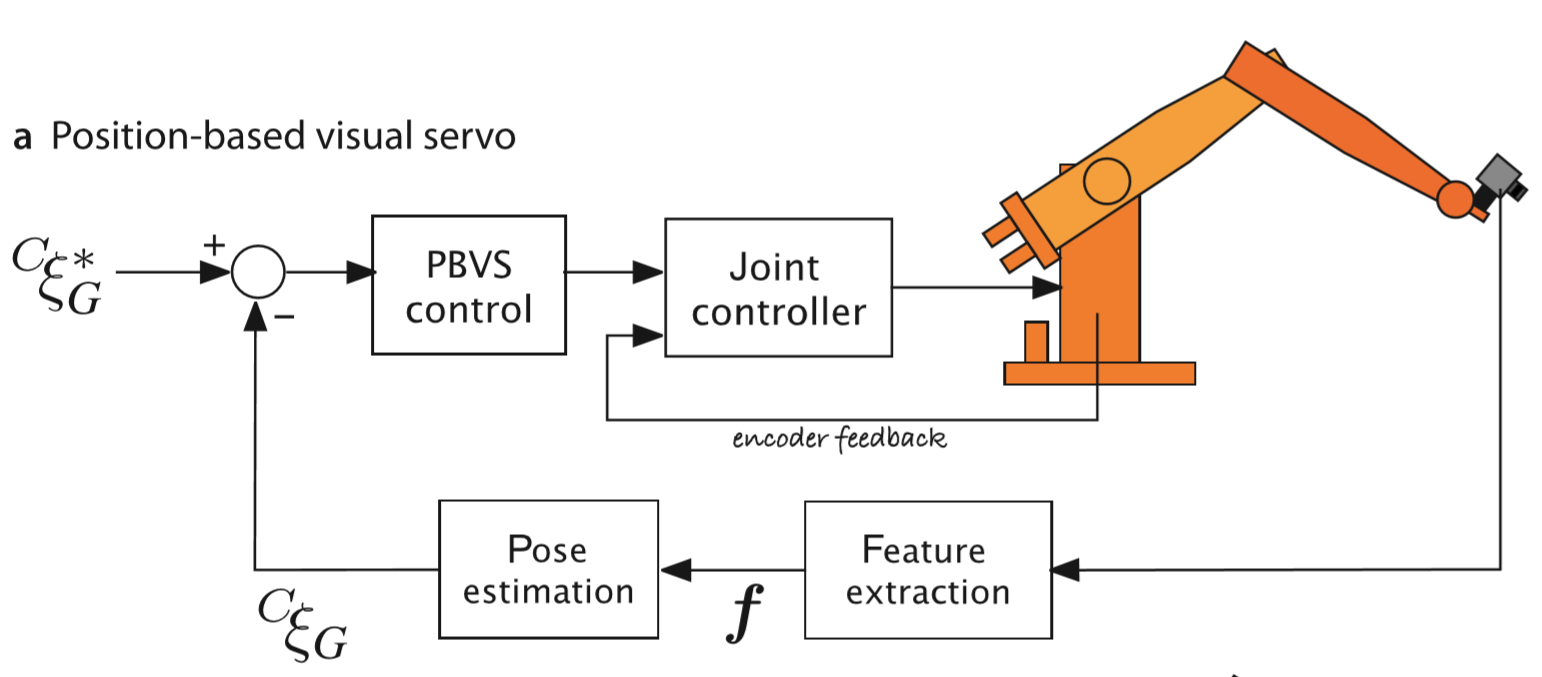
\includegraphics[width=.8\linewidth]{Figures/PBVScontrolscheme}
		\caption{Position Based Visual Servoing control scheme}
		\label{fig:PBVScontrolscheme}
	\end{center}
\end{figure}

Using our feature extractor we obtain a point correspondences which relates world points \textit{P} to image plane points \textit{p}: 

\begin{align*}
	\mathbf{P}_{n} = 
	\begin{bmatrix} 
	X_{1} & Y_{1} & Z_{1}  \\
	X_{2} & Y_{2} & Z_{2}  \\
	\vdots & \vdots & \vdots\\
	X_{n} & Y_{n} & Z_{n}  
	\end{bmatrix} & &
	\mathbf{p} = 
	\begin{bmatrix} 
	u_{1} & u_{2} &  \dots & u_{n}  \\
	v_{n} & v_{2} & \dots & v_{n}  
	\end{bmatrix}
\end{align*} 

This correspondence can then be substituted into a pose estimator, which gives the pose of the camera with respect to the world points $\prescript{CAM}{}{\mathbf{T}}_{P}$. Given a desired camera pose with respect to the object $\prescript{CAM^{*}}{}{\mathbf{T}}_{P}$ , the desired camera transformation can be defined as:

\begin{equation}
	\begin{aligned}
	\prescript{CAM}{}{\mathbf{T}}_{CAM^{*}} & =
	\prescript{CAM}{}{\mathbf{T}}_{P}  \prescript{P}{}{\mathbf{T}}_{CAM^{*}}\\
	 & = \prescript{CAM}{}{\mathbf{T}}_{P}  \prescript{CAM^{*}}{}{\mathbf{T}}_{P}^{-1}
	\end{aligned}	
\end{equation}


This can be used to compute a desired camera velocity $\delta \mathbf{T}_{CAM}$ which is scaled by a control gain $\lambda$. This allows for incremental motions:

\begin{equation}
	{\mathbf{T}_{CAM}}_{(k+1)} = {\mathbf{T}_{CAM}}_{(k)} + {\delta \mathbf{T}_{CAM}}_{(k)} \lambda
\end{equation}

This can also be expressed as a desired velocity of the camera $\mathbf{v}_{CAM}$
To use this desired velocity in our joint controller, it needs to be transformed from a velocity with respect to the cameras coordinate frame to a velocity with respect to the origin. This can be done using an adjoint transformation (Appendix \ref{Adjoint transformation}):

\begin{equation}
	\prescript{0}{}{\mathbf{ADJ}}_{CAM} = \\
	\begin{bmatrix}
		\prescript{0}{}{\mathbf{R}}_{CAM} & \prescript{0}{}{\mathbf{\hat{t}}}_{CAM}\prescript{0}{}{\mathbf{R}}_{CAM} \\
		\mathbf{0} & \prescript{0}{}{\mathbf{R}}_{CAM} 
	\end{bmatrix}
\end{equation}


which can be used to compute:

\begin{equation}
	\prescript{}{\{0\}}{\mathbf{V}}_{CAM} =
	\prescript{0}{}{\mathbf{ADJ}}_{CAM} \prescript{}{\{CAM\}}{\mathbf{V}}_{CAM}
\end{equation}

thus, the desired velocity can be provided to the joint controller as:

\begin{equation}
	\mathbf{x}_{d} = \mathbf{x}_{e} + {\mathbf{V}}_{CAM} 
\end{equation}


%%%%%%%%%%%%%%
\subsection{Image Based Visual Servoing}\label{Image Based Visual Servoing}

Image Based Visual Servoing(IBVS) contrasts PBVS by computing its control signal entirely in the image space, as shown by its control scheme in Figure \ref{fig:IBVScontrolscheme}. 

\begin{figure}[H]
	\begin{center}
		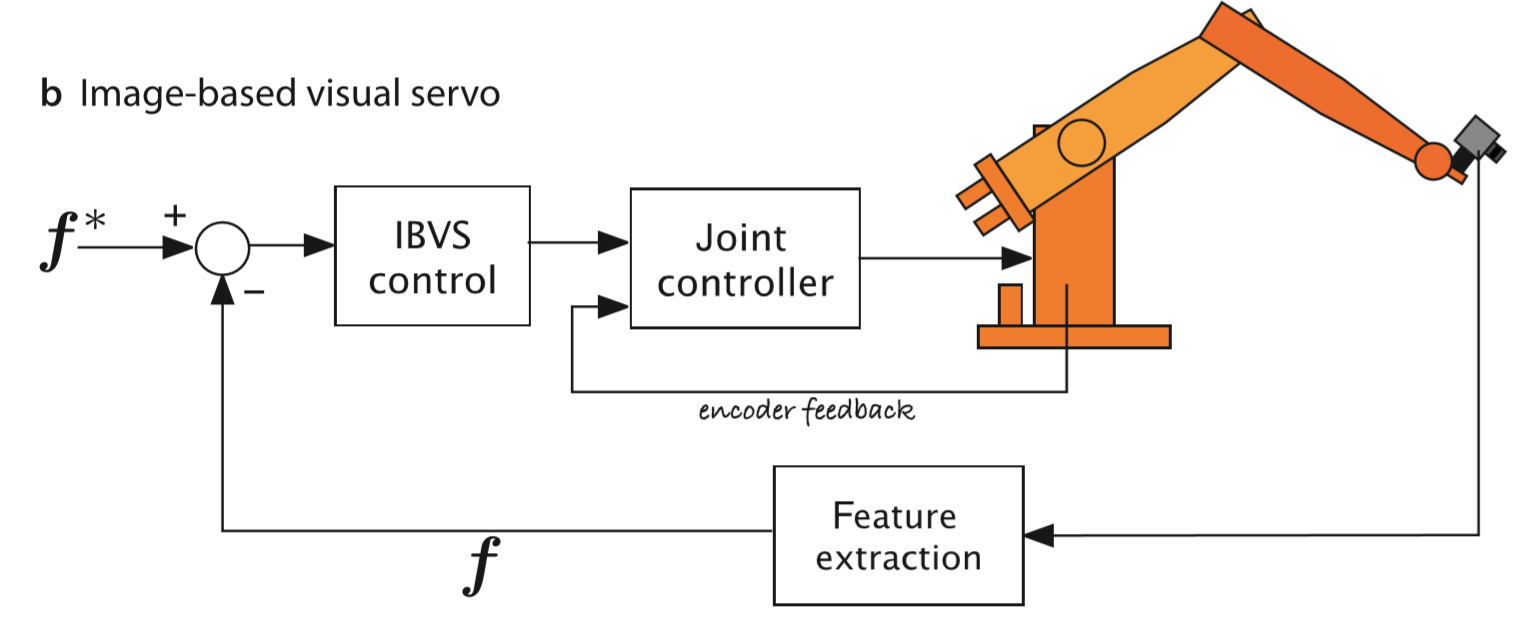
\includegraphics[width=.8\linewidth]{Figures/IBVScontrolscheme}
		\caption{Image Based Visual Servoing control scheme}
		\label{fig:IBVScontrolscheme}
	\end{center}
\end{figure}

As before, world points \textit{P} project to image points \textit{p} given a camera pose $T_{CAM}$. Similarly, a desired camera pose $T_{CAM^{*}}$ will project world points \textit{P} project to image points $p^{*}$. Using this relationship, IBVS aims to move the pixel points $p$ to their corresponding goals $p^{*}$, thus implicitly moving the robot to a desired pose $T_{CAM^{*}}$.	

To perform this control, a method to relate motion in cartesian space to motion in image space is required. This relationship is called the Interaction matrix or, as already defined in this project, the Image Jacobian \ref{Image Jacobian}. The equation \ref{imagejacobianequationstacked} can be rearranged to give, for \textit{n} feature points:

\begin{equation}
	\label{imagejacobianequation}
	\mathbf{\nu} = \\
	{\begin{bmatrix} 
		J_{p}(p_{1} , Z_{1})   \\
		J_{p}(p_{2} , Z_{2})   \\
		\vdots \\
		J_{p}(p_{n} , Z_{n})
	\end{bmatrix}}^{-1} \\ 
	\begin{bmatrix} 
		u_{1} \\
		v_{1}  \\
		u_{2} \\
		v_{2}  \\
		\vdots\\
		u_{n} \\
		v_{n}  \\  
	\end{bmatrix} \\	
\end{equation} 

This gives us the camera velocity required to achieve a desired motion of the image feature. The simplest way to prescribe this desired motion is to use a simple linear controller 

\begin{equation}
	\mathbf{\dot{p}^{*}} = \lambda(\mathbf{p^{*}} - \mathbf{p})
\end{equation}

And substitute it into equation \ref{imagejacobianequation} to give:

\begin{equation}
	\label{velocityimagejacobian}
	\mathbf{\nu} = \\
	\lambda{\begin{bmatrix} 
		J_{p}(p_{1} , Z_{1})   \\
		J_{p}(p_{2} , Z_{2})   \\
		\vdots \\
		J_{p}(p_{n} , Z_{n})
	\end{bmatrix}}^{-1} \\ (\mathbf{p^{*}} - \mathbf{p})		
\end{equation} 

As the matrix is not square when using the 4 feature points extracted in Section (\ref{Feature Point Extraction}), the inverse must be computed using the pseudo inverse (Appendix \ref{Pseudoinverse}) which is denoted by \textsuperscript{+}. This results in a velocity that \textit{minimises the norm of the feature velocity error}.

The image jacobian is a first order approximation of the relationship between camera motion and feature points motion. Using a second order approximation will result in faster convergence, and it can be found by taking the \textit{mean} of the pseudo inverse at the current and desired location:

\begin{equation}
\label{meanvelocityimagejacobian}
\mathbf{\nu} = \\
	\lambda/2 \\
	\begin{bmatrix}
	{\begin{bmatrix} 
	J_{p}(p_{1} , Z_{1})   \\
	J_{p}(p_{2} , Z_{2})   \\
	\vdots \\
	J_{p}(p_{n} , Z_{n}) \\
	\end{bmatrix}}^{+} +
	{\begin{bmatrix} 
	J_{p}(p^{*}_{1} , Z^{*}_{1})   \\
	J_{p}(p^{*}_{2} , Z^{*}_{2})   \\
	\vdots \\
	J_{p}(p^{*}_{n} , Z^{*}_{n}) \\
	\end{bmatrix}}^{+} \\
	\end{bmatrix} \\
	(\mathbf{p^{*}} - \mathbf{p})		
\end{equation} 

This velocity is then transformed using an adjoint transformation, as shown in Section \ref{PBVS}, to give a velocity in the origin frame. This can once again be inputted to a suitable joint controller.

%%%%%%%%%%%%%%%%%%%%%%%%%%%%%%%%%%%%%%%%%
\subsection{Simulation}

Animated simulation's can be found in the project \href{https://github.com/Hashkhan98/Vision-Based-Control-of-an-Industrial-Robotic-Manipulator}{repository}. 

\begin{figure}[H]
	\begin{center}
		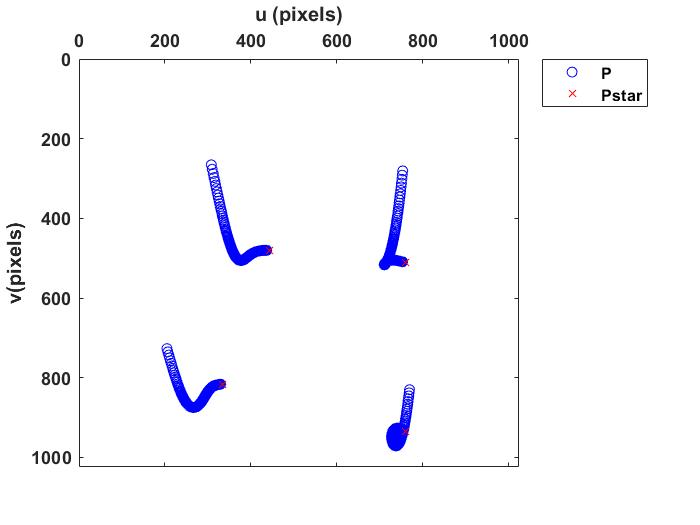
\includegraphics[width=.7\linewidth]{Figures/IBVSimagespace}
		\caption{The motion of points in the image space using IBVS}
		%		\label{}
	\end{center}
\end{figure}

\begin{figure}[H]
	\begin{center}
		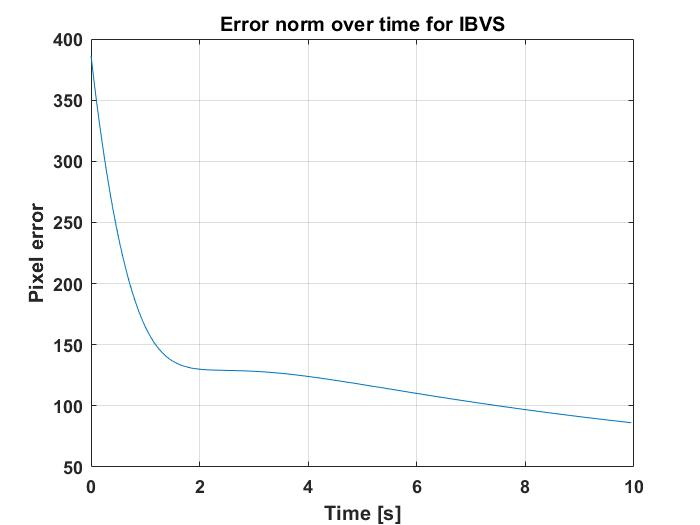
\includegraphics[width=.7\linewidth]{Figures/IBVSerrorplot}
		\caption{IBVS norm of \textit{pixel error} over time}
		%		\label{}
	\end{center}
\end{figure}

\begin{figure}[H]
	\begin{center}
		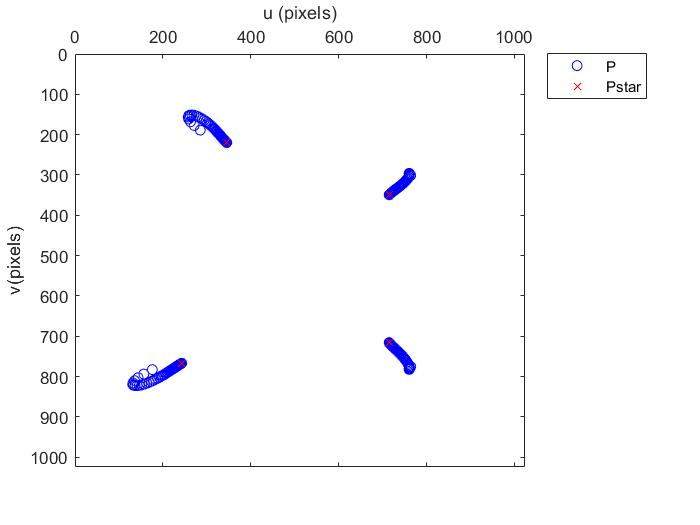
\includegraphics[width=.7\linewidth]{Figures/PBVSimagespace}
		\caption{The motion of points in the image space using PBVS}
		%		\label{}
	\end{center}
\end{figure}

\begin{figure}[H]
	\begin{center}
		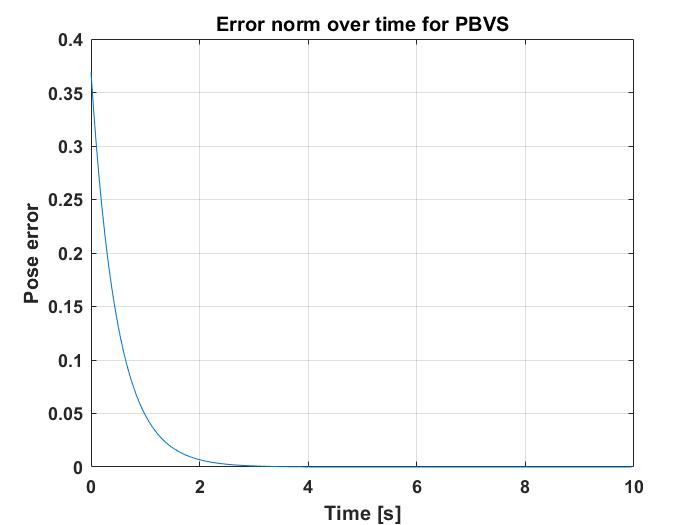
\includegraphics[width=.7\linewidth]{Figures/PBVSerror}
		\caption{PBVS norm of \textit{pose error} over time}
		%		\label{}
	\end{center}
\end{figure}

Performing this task on hardware requires \textit{system integration} and is outlined in the following section.
 
%%%%%%%%%%%%%%%%%%%%%%%%%%%%%%%%%%%%%%%%%%%%%%%%%
\newpage
\section{Implementation}\label{Implementation}

This section outlines how the theory was applied on hardware. It provides a workflow that \textit{integrates} the subsystems discussed in previous sections,results regarding the pick and place task and suggests future recommendations.

%%%%%%%%%%%%%%%%%%%%%%%%%%%%%%%%%%%%%%%%%%%%%%%%%
\subsection{Workflow}

An overview of the workflow used to integrate the systems is providing, relying heavily on the architecture of PBVS (Figure \ref{{fig:PBVScontrolscheme}}) and IBVS (Figure \ref{fig:IBVScontrolscheme}). Common to both formulations is obtaining a desired pose relative to the target object, as shown in Figure \ref{fig:definegoalpose}.

\begin{figure}[H]
	\begin{center}
		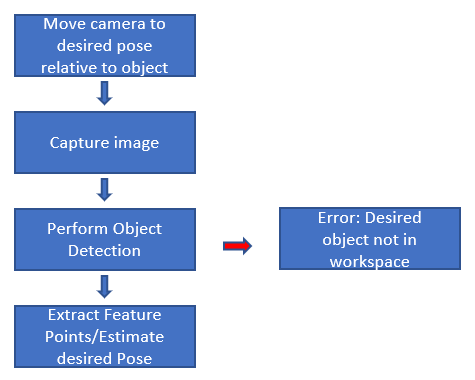
\includegraphics[width=.6\linewidth]{Figures/Definegoalpose}
		\caption{Workflow for defining a desired relative pose.}
		\label{fig:definegoalpose}
	\end{center}
\end{figure}

If the desired object is not detected in the image using our \textit{Faster-RCNN}, an error is reported.\

Then either position-Based visual servoing (Figure \ref{fig:PBVSworkflow}) or image based visual servoing (Figure \ref{fig:IBVSworkflow}) is performed.

\begin{figure}[H]
	\begin{center}
		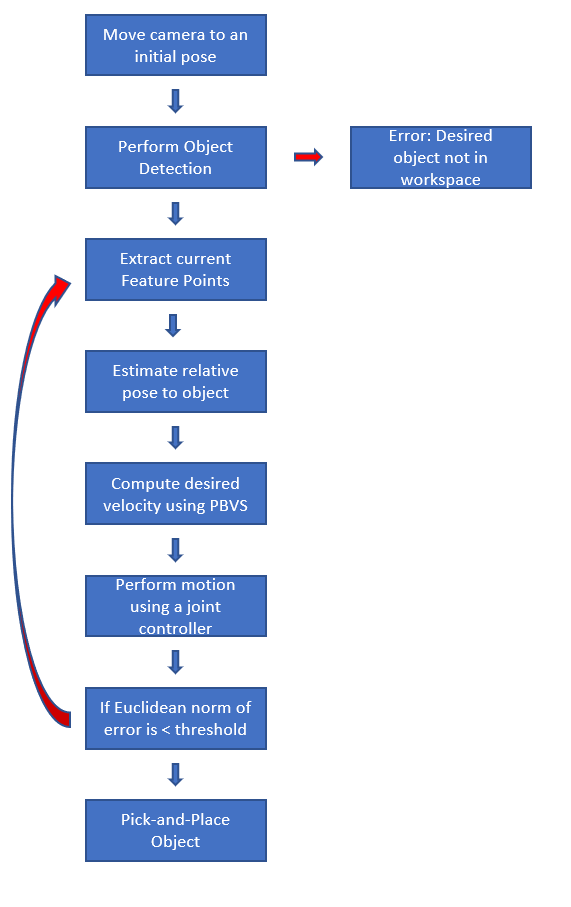
\includegraphics[width=.6\linewidth]{Figures/PBVSworkflow}
		\caption{Workflow for PBVS.}
		\label{fig:PBVSworkflow}
	\end{center}
\end{figure}

\begin{figure}[H]
	\begin{center}
		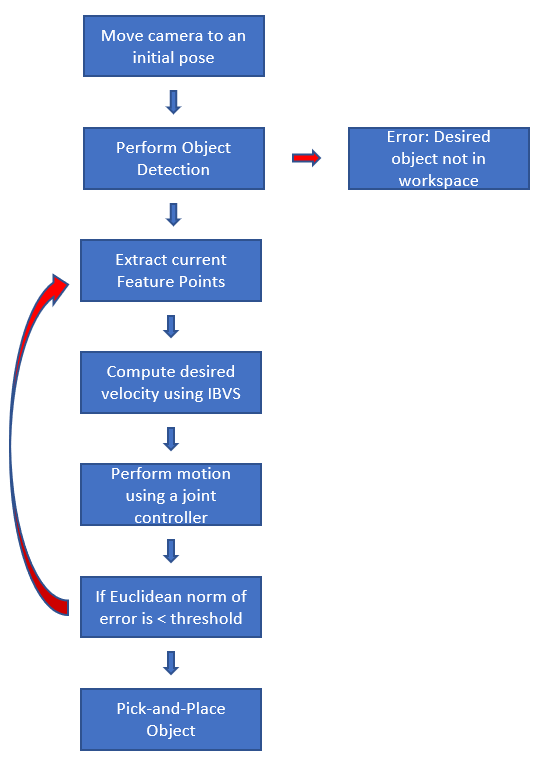
\includegraphics[width=.6\linewidth]{Figures/IBVSworkflow}
		\caption{Workflow for IBVS.}
		\label{fig:IBVSworkflow}
	\end{center}
\end{figure}

where the key difference is whether the task is prescribed in the \textit{image} or \textit{Cartesian} space. Once the error between the current and desired pose falls below a certain threshold, a series of fixed joint movements \textit{relative to the current joint angles} are performed to lower down, grasp, lift and then place the object and then the robot is shut-down. This workflow allows thus integrates our \textit{subsystems} to perform a pick-and place task. 
Using this workflow achieved the following results.

%%%%%%%%%%%%%%%%%%%%%%%%%%%%%%%%%%%%%%%%%%%%%%%%%
\subsection{Results}\label{Results}

A successful demonstration of the pick-and-place task using IBVS control can be visualised in the project \href{https://github.com/Hashkhan98/Vision-Based-Control-of-an-Industrial-Robotic-Manipulator}{repository}.

Figure \ref{fig:IBVSerrorproof} \textit{highlights} a reduction in \textit{pixel error} corresponding to a reducing \textit{pose error}.

\begin{figure}[H]
	\begin{center}
		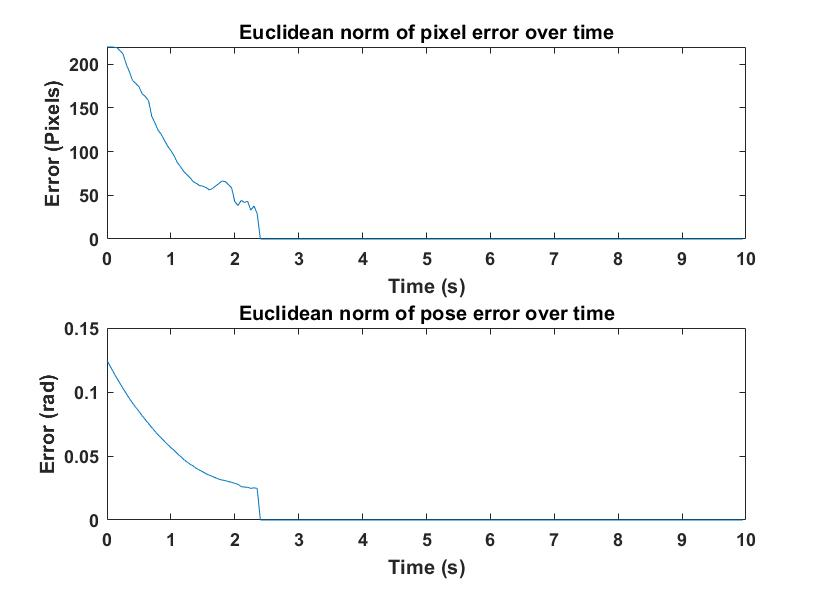
\includegraphics[width=.99\linewidth]{Figures/IBVSerrorproof}
		\caption{Results for IBVS implemented on hardware}
		\label{fig:IBVSerrorproof}
	\end{center}
\end{figure}

These results will now be discussed in detail and future recommendations made.

%%%%%%%%%%%%%%%%%%%%%%%%%%%%%%%%%%%%%%%%%%%%%%%%%
\subsection{Discussion and Future Recommendations}


This project successfully leveraged IBVS and a Faster-RCNN to achieve it's objective. This section provides context for how this was done and suggests future recommendations to improve the workflow.\

First and foremost, the 5DOF robot arm was not suitable for the task as it did not have enough \textit{torque} or manipulability to \textit{effectively} implement the workflow designed with a 6DOF manipulator in mind. It is recommended this workflow should either be altered to find better control strategies specific to the 5DOF robot arm or be implemented on a suitable 6DOF arm.\

Additionally, the 5DOf arm's limited manipulability range combined with the available webcams substandard \textit{field of view (fov)} restricted the \textit{effective} workspace since both the \textit{current} and \textit{desired} image feature points must be \textit{concurrently} present in the image to initialise the IBVS workflow. This limitation could be overcome by using a larger robot or a camera with a fish-eye lens providing a large \textit{fov}.  

As elaborated in Appendix \ref{App:Alternative Cameras}, other cameras were proposed for this project (including a model with a suitable fish-eye lens) but were not implemented due to various limitations.

The object detector is currently implemented in Python Tensorflow. A future recommendation is to retrain the classifier using Matlab to simplify integration and implementation.


%%%%%%%%%%%%%%%%%%%%%%%%%%%%%
\newpage
\section{Conclusion}\label{sec:Conclusion}

As outlined by the Objective (\ref{Objective}), the goal of this project was to pick-and-place task a desired object using a robotic manipulator with an eye-in-hand camera. This task was successfully implemented using a image based visual servoing controller (\ref{Results}).\
This was achieved by simplifying this task into various subsystems.\

First, a mathematical model was required to understand and control the kinematics of a robotic manipulator. This was done by relating the motion of robotic \textit{joints} to the subsequent movement of it's \textit{end-effector}, leading to the development of a inverse kinematic controller.\

Then, a camera model was used to relate 3-dimensional objects to their \textit{projection} in a 2-dimensional image. The \textit{Intrinsic parameters} of a camera were found through \textit{camera calibration} and this allowed us to perform \textit{pose estimation}. Additionally, a technique for extracting \textit{feature points} was established and the mapping of their motion from image to Cartesian space was described using an \textit{image jacobian}. \

Subsequently, artificial neural networks were introduced in the context of machine vision. This was used to provide insight into training a \textit{Faster Region-based Convolutional Neural Network} by applying \textit{transfer learning} on a pre-trained model. This resulted in a robust model able to perform in challenging conditions.\

Then, pose estimation was used to formulate a \textit{Position Based Visual Servoing} controller while the image jacobian formed the bedrock of a Image Based Visual Servoing controller. The applicability of these techniques was discussed in the context of this project. \


Finally, the prior subsystems were integrated on hardware and the project's primary objective was achieved. The various techniques utilised in this project and the hardware limitations faced were discussed and future recommendations were suggested to potentially improve this implementation.\

Ultimately, this project explored a few aspects of a challenging control problem and can conceivably form the foundation for further work by future students at the University of Newcastle. 



%%%%%%%%%%%%%%%%%%%%%%%%%%%%%%%%
\newpage
\bibliographystyle{harvard}
\bibliography{References} % This is the .bib file where the bibliography database is stored
%%%%%%%%%%%%%%%%%%%%%%%%%%%%%%
\newpage
\appendix

\section{Time Log}\label{Time Log}

\begin{figure}[H]
	\begin{center}
		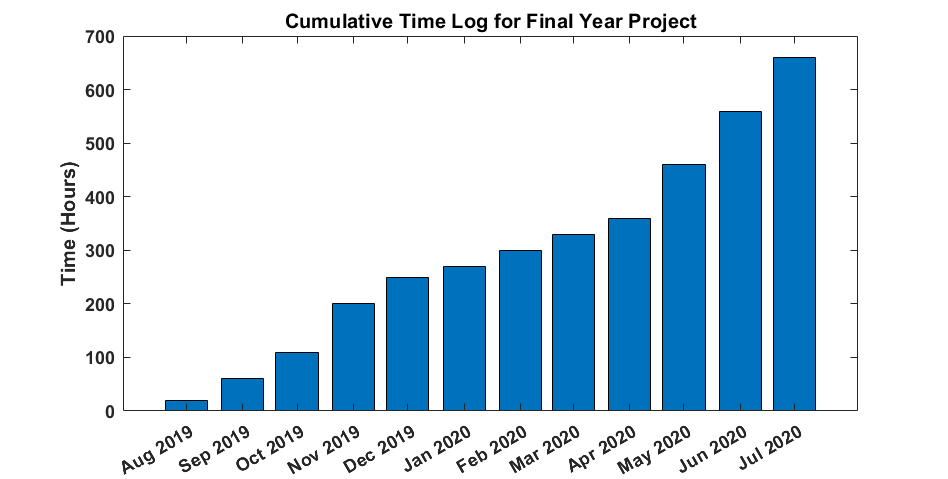
\includegraphics[width=1\linewidth]{Figures/TimeLog}
		\caption{Cumulative Time Log}
		\label{fig:TimeLog}
	\end{center}
\end{figure}

\section{Engineers Australia Competencies}
Undertaking this project allowed me to develop competency in the following areas, as required by the "Stage 1 Competency Standard for Professional Engineer" by Engineers Australia.
\subsection{Knowledge and Skill Base} 
This project has developed my understanding of mathematical modelling of physical systems and control theory. It also increased my skills in programming and ability to solve real-world problems.

\subsection{Engineering Application Ability}

I utilised the engineering method to solve a complex problem by dividing it into simpler sub-problems. I then tackled each sub-problem by researching suitable techniques, synthesising viable solutions and iteratively testing and improving them. 

\subsection{Professional and Personal Attributes}

This project allowed me to improve my project management skills, progressing multiple codependent tasks and finding feasible solutions to a plethora of issues. I also honed my ability to learn new skills through independent research and developed an appreciation for effective communication of complex ideas.   


%%%%%%%%%%%%%%%%%%%%%%%%%%%%%
\newpage
\section{Industrial Application}\label{Industrial Application}

The following provides an example of an application of Visual-servoing used in industry. \\ 

Ampcontrol CSM is a site that manufactures and assembles various electrical systems. Many of these systems contain printed circuit boards, which require a layer of protective coating to protect them from harsh environments that may contain high humidity, varying temperatures and airborne particles that may disrupt the circuits functionality. \


The current approach to conformal coating on-site is to perform a bulk spray of several printed circuit boards (PCBs) using an aerosol can of polyurethane coating. This process involves covering parts, such as pins, connectors and potentiometers that must be coating-free to remain functional, with tape and vinyl coating. These are then placed in a well-ventilated room, bulk sprayed by production staff and then left to cure overnight. The tape and vinyl are then removed, and the board is inspected. \


This process is labour intensive and exposes workers to potentially hazardous fumes. Therefore, an alternative method was proposed and developed which aimed to automate the process. \


This method uses a pneumatic nozzle attached to a \textit{Techman Robot TM5-900} collaborative robot arm to autonomously spray the desired PCBs while avoiding parts that must remain coating free. \


The developed workflow allows the designation of a desired board are that needs to be coated as a mechanical layer in Altium (industrial PCB design software). This is then converted to a \textit{tool-path} and simulated through RoboDK (Robotics modelling software) for verification. \
The specified tool-path can then be used to guide the robot arm and operate it's pneumatic dispenser to coat a desired PCB.\


The pneumatic dispenser's accuracy, and thus the success of the entire task, is dependent on precise knowledge of the board's position and orientation. This could not practically be achieved through the use of jigs as there were hundred's of different board shapes and sizes. Therefore, visual-servoing was used to \textit{align} the dispenser to the board. This was achieved by using Techman Robot's proprietary \textit{Tmflow} software which has a visual-servoing implementation.\

The robot arm successfully demonstrated the task as a proof of concept, highlighting the potential of vision-based control in industry.

\section{Adjoint transformation}\label{Adjoint transformation}

The adjoint transformation was defined by \cite{Banavar2008} and is used to transform a velocity $\prescript{B}{}{\mathbf{\nu}} = [\prescript{B}{}{\mathbf{v}} , \prescript{B}{}{\mathbf{\omega}}]^{\top}$from the basis frame $\{B\}$ to the basis frame $\{A\}$. This is achieved through the relationship:

\begin{equation}
	\begin{split}
		\begin{bmatrix}
			\prescript{A}{}{\mathbf{v}} \\ \prescript{A}{}{\mathbf{\omega}}
		\end{bmatrix}
		& = \
		\begin{bmatrix}
			\prescript{A}{}{\mathbf{R}}_B & \prescript{A}{}{\hat{\mathbf{t}}}_B \prescript{A}{}{R}_B \\
			\mathbf{0}^{3 \times 3}	& \prescript{A}{}{\mathbf{R}}_B
		\end{bmatrix} 
		\begin{bmatrix}
			\prescript{B}{}{\mathbf{v}} \\ \prescript{B}{}{\mathbf{\omega}}
		\end{bmatrix} \\
		\prescript{A}{}{\mathbf{\nu}} & = \mathbf{Ad}(\prescript{A}{}{\mathbf{T}}_B) \prescript{B}{}{\mathbf{\nu}}
		\end{split}
\end{equation}

where $\prescript{A}{}{\hat{\mathbf{t}}}_B$ indicates the \textit{skew} of the translation vector $ \prescript{A}{}{\mathbf{t}}_B = [\prescript{A}{}{X}_B , \prescript{A}{}{Y}_B , \prescript{A}{}{Z}_B]^{\top} $ as:

\begin{equation}
	\prescript{A}{}{\hat{\mathbf{t}}}_B = 
	\begin{bmatrix}
		0          & \prescript{A}{}{Z}_B         & \prescript{A}{}{Y}_B  \\
		\prescript{A}{}{Z}_B   & 0  		   & -\prescript{A}{}{X}_B  \\
		-\prescript{A}{}{Y}_B  & -\prescript{A}{}{X}_B  & 0 
	\end{bmatrix} 
\end{equation}

and $\mathbf{Ad}(\prescript{A}{}{\mathbf{T}}_B)$ is \textit{adjoint transform} expressed as a function of the desired basis transformation.



\section{Moore-Penrose Inverse}\label{Pseudoinverse}

The Moore-Penrose inverse is defined by \cite{moore1920reciprocal} and \cite{penrose1955generalized}. They state, given a matrix $\mathbf{A}$ whose rows are linearly independent:

\begin{equation}
	\mathbf{A}^{+} = \mathbf{A}^{\top}(\mathbf{A} \mathbf{A}^{\top})^{-1}
\end{equation}

Where $\mathbf{A}^{+}$ is the \textit{right inverse} as $\mathbf{A}	\mathbf{A}^{+} = \mathbf{I}$. \\
This is known as a \textit{pseudoinverse} and is denoted by $^{+}$. In cases where a matrix is not invertible (non-square), the pseudoinverse provides a least squares approximation of its inverse and is implemented by the \texttt{pinv} function in Matlab.



%%%%%%%%%%%%%%%%%%%%%%%%%%%%%%%%%%%%%%%
\section{Optimisation of sorting problem}

When performing a pick and place problem for multiple objects, we can represent the task as having items $ D = [A,B,C]$ at initial positions $\{\mathbf{d}_0\}$ and having desired locations $\mathbf{d}^*$. If the order in which these items are picked and place matters, then there is no further work required. However, if the \textit{order does not matter}, then it is purported there must be an optimal method for sorting these objects that minimises the \textit{total displacement} of the end effector. \

Fortunately, this task can be formulated as a subset of the \textit{travelling salesman problem} and a solution can be found using a linear optimiser. \

This was implemented in Matlab using \texttt{intlinprog} as shown by Figure \ref{fig:travellingsalesman}. 

\begin{figure}[H]
	\begin{center}
		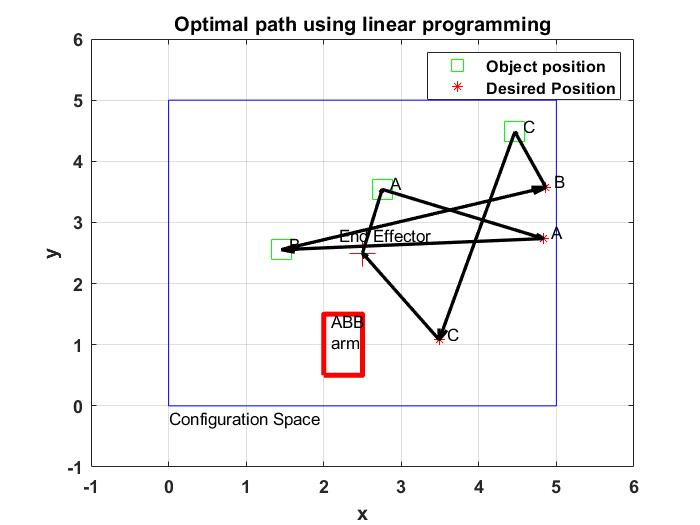
\includegraphics[width=.6\linewidth]{Figures/optimalpath}
		\caption{The optimal path to sort objects $[A,B,C]$ to desired locations $[A*,B*,C*]$}
		\caption{A minimal displacement path using linear programming}
		\label{fig:travellingsalesman}
	\end{center}
\end{figure}

It was intended for this work to be extended to 3 dimensions and form part of a trajectory generator using bezier curves \citep{choi2008path}.


%%%%%%%%%%%%%%%%%%%%%%%%%%%%%%%%%%%%%%%
\section{Euler Angles}\label{App:Euler Angles}

Rotation matrices are non-minimal representations of orientation and have redundant parameters. For the special orthogonal group (SO3), 3 parameters can be used to provide a minimal representation \cite{siciliano2010robotics}. \\

Following the Roll-Pitch-Yaw (RPY) convention used in aeronautics, rotations are considered to occur, \textbf{in order}, about the z , y and x axis. Rotations can be denoted as roll ($\phi$), pitch ($\theta$) and yaw ($\psi$). The rotation matrix \ref{eqn:rotationmatrix} can now be expressed as, for $\theta$ in the range $(\dfrac{-\pi}{2} , \dfrac{\pi}{2})$:

\begin{equation}
	\mathbf{\Theta} =
	\begin{bmatrix}
	\phi \\ \theta \\\psi 
	\end{bmatrix}
	= 
	\begin{bmatrix}
	atan2(-R_{31} , \sqrt{R_{33}^{2} + R_{33}^{2}}) \\
	atan2(R_{21} , R_{11}) 
	\end{bmatrix}
\end{equation}

and for $\theta$ in the range $(\dfrac{\pi}{2} , \dfrac{3\pi}{2})$:
\begin{equation}
	\begin{bmatrix}
	\phi \\ \theta \\\psi 
	\end{bmatrix}
	= 
	\begin{bmatrix}
	atan2(R_{32} , R_{33}) \\
	atan2(-R_{31} , \sqrt{R_{33}^{2} + R_{33}^{2}}) \\
	atan2(R_{21} , R_{11}) 
	\end{bmatrix}
\end{equation}

%%%%%%%%%%%%%%%%%%%%%%%%%%%%%%%%%%%%%%%
\section{Alternative Cameras}\label{App:Alternative Cameras}

The first camera considered for use during this project was a \textit{Point Gray chameleon cmln-13s2c} camera with a fish-eye lens. Due to it's protective casing limiting its field of view, low frame-rate and poor picture quality when interfaced with Matlab (Figure \ref{fig:chameleoncameraimage}), this camera was deemed unfit for the task.\\

\begin{figure}[H]
	\begin{center}
	\centering

	\subfloat[The camera's standard case (protective casing not shown), retreived from \cite{FlirSystems} ]{{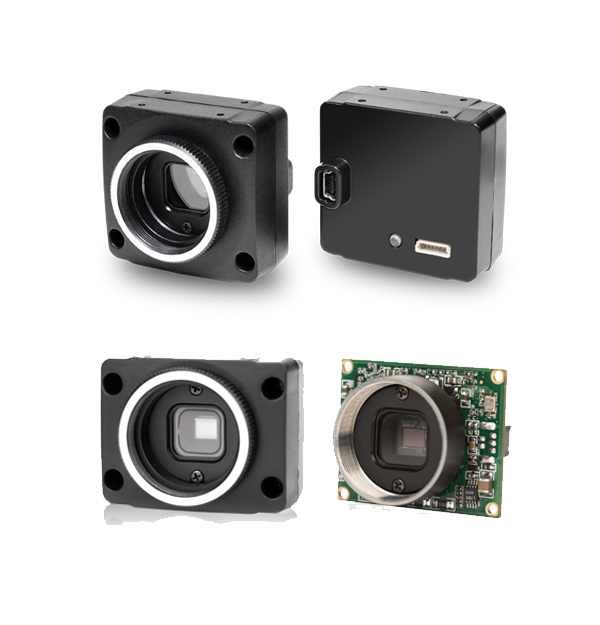
\includegraphics[scale=.3]{Figures/chameleoncamera} }}%
	\hfil
	\subfloat[Example of captured image]{{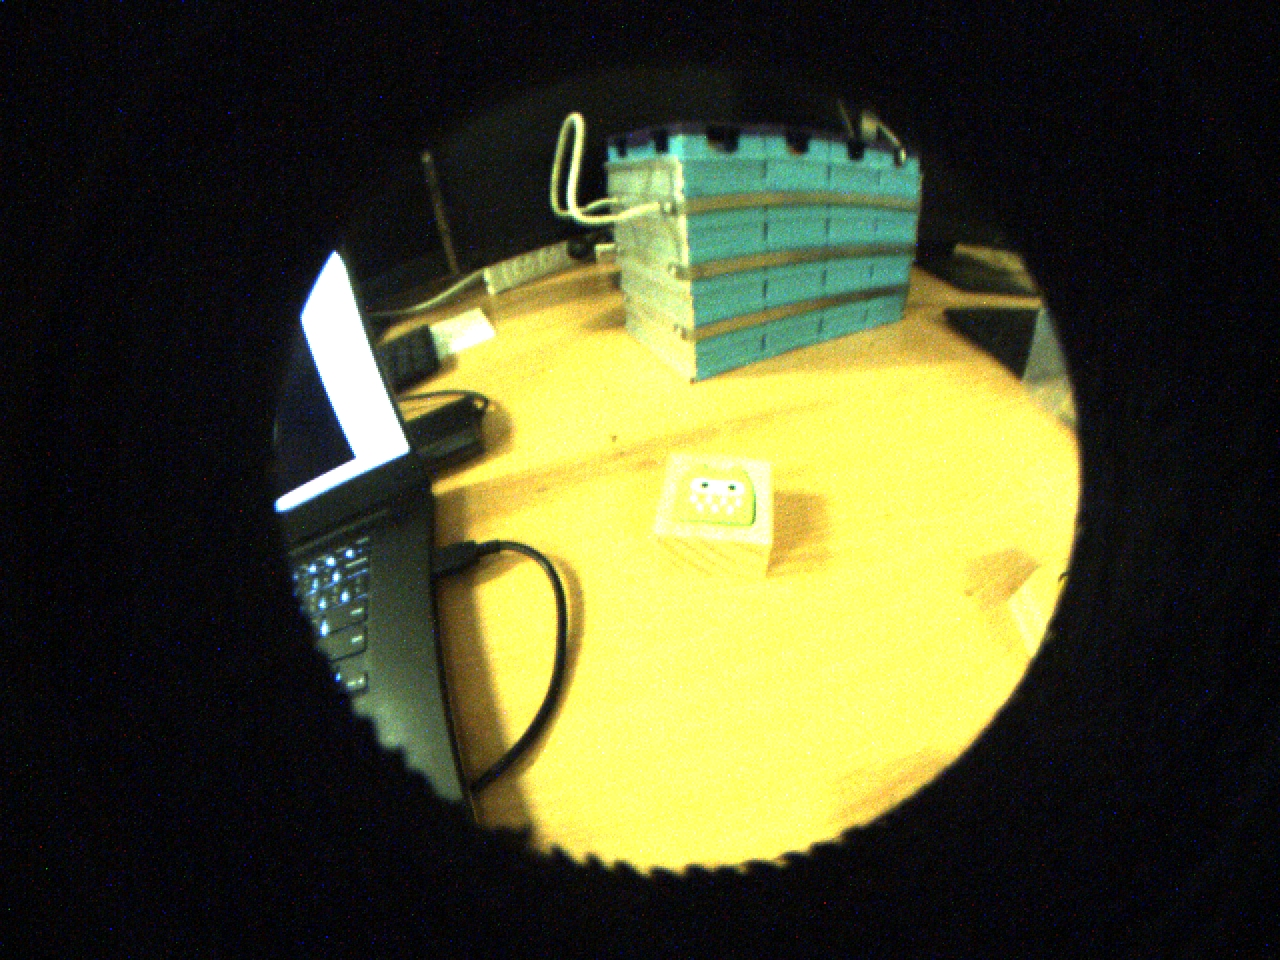
\includegraphics[scale=.2]{Figures/chameleoncameraimage} }}%
	
	\caption{The Point Gray chameleon cmln-13s2c}%
	\label{fig:chameleoncameraimage}%
	\end{center}
\end{figure}

Therefore, a \textit{Raspberry Pi Zero W} intefaced with a \textit{Raspberry Pi Camera Board v2} was acquired. This setup provided a high resolution (1280x720) image at 60fps and could be directly interfaced with Matlab. This camera was used to generate the training and validation dataset for object detection and was also calibrated using camera calibration. \


Unfortunately, a suitable mount to integrate it with the 5DOF robot arm was not manufactured due to time constraints and weight concerns due to actuator torque limits. \


Thus, the Microsoft webcam was used as it could be easily mounted to the robot and was light enough to minimise joint current overloading. 


%
%
%\begin{equation*}
%\mathbf{J} =
%\begin{bmatrix}
%J_{v} \\ J_{\omega}  
%\end{bmatrix}
%\end{equation*}\
%
%\begin{equation*}
%\mathbf{k}(\mathbf{q}) = \mathbf{x_{e}}=  
%\begin{bmatrix}
%x \\ y \\ z \\ \phi \\ \theta \\ \psi 
%\end{bmatrix}
%\end{equation*}\
%
%\begin{equation*}
%\mathbf{q} =
%\begin{bmatrix}
%q1 \\ q2 \\ q3 \\ q4  
%\end{bmatrix}
%\end{equation*}\
%
%\begin{equation*}
%\mathbf{\prescript{A}{}T_{B}} =
%\begin{bmatrix}
%\mathbf{R}  & \mathbf{t} \\
%\boldmath{0}  & 1  
%\end{bmatrix}.
%\end{equation*} \
%
%\begin{equation*}
%\mathbf{R} =
%\begin{bmatrix}
%R11  & R12 & R13 \\
%R21  & R22 & R23 \\
%R31  & R32 & R33 
%\end{bmatrix}.
%\end{equation*} \
%
%\begin{equation*}
%\mathbf{t} =
%\begin{bmatrix}
%x  \\ y \\ z \\
%\end{bmatrix}.
%\end{equation*} \
%
%\begin{equation}
%\mathbf{\prescript{0}{}T_{EE}} = \mathbf{\prescript{0}{}T_{1}}\mathbf{\prescript{1}{}T_{2}}\\
%\mathbf{\prescript{2}{}T_{3}}\mathbf{\prescript{3}{}T_{EE}}
%\end{equation} 
%
%
%\begin{equation*}
%\begin{bmatrix}
%\mathbf{\nu} \\ \mathbf{\omega} 
%\end{bmatrix}
%=
%\mathbf{J_{A}(q)} \mathbf{\dot{q}}
%\end{equation*}\
%
%
%\begin{equation*}
%\mathbf{e = xd - xe}
%\end{equation*}\
%
%\begin{equation*}
%\mathbf{x_{e}} =
%\begin{bmatrix}
%x  \\ y \\ z \\ \theta
%\end{bmatrix}.
%\end{equation*} \
%
%\begin{equation*}
%dim \,\mathbf{xe} > dim\,\mathbf{ q}
%\end{equation*}\
%
%\begin{equation}
%\mathbf{\prescript{0}{}T_{CAM}} = \mathbf{\prescript{0}{}T_{EE}}\mathbf{\prescript{EE}{}T_{CAM}}\\
%\end{equation} 
%
%\begin{equation}
%\mathbf{\prescript{CAM}{}T_{P}} = \mathbf{\prescript{0}{}T_{EE}}\mathbf{\prescript{EE}{}T_{CAM}}\\
%\end{equation} 
%
%\begin{equation}
%\mathbf{\prescript{P}{}T_{P*}} = \mathbf{\prescript{CAM}{}T_{P}}\mathbf{\prescript{P}{}T_{P*}}\\
%\end{equation} 
%
%
%\begin{equation*}
%\mathbf{P} =
%\begin{bmatrix}
%\mathbf{X}  \\ \mathbf{Y} \\ \mathbf{Z} 
%\end{bmatrix}.
%\end{equation*} \
%
%
%\begin{equation*}
%\mathbf{P} =
%\begin{bmatrix}
%\mathbf{X}  \\ \mathbf{Y} \\ \mathbf{Z} 
%\end{bmatrix}.
%\end{equation*} \
%
%\begin{equation*}
%\mathbf{e} =
%\mathbf{p*} - \mathbf{p}
%\end{equation*} \
%
%
%\begin{equation*}
%\begin{aligned}
%\mathbf{e} =\mathbf{p*} - \mathbf{p} \\
%\mathbf{\dot{e}} = \mathbf{\nu} = \mathbf{p*} - \mathbf{p}
%\end{aligned}
%\end{equation*} \
%
%\begin{equation*}
%\begin{aligned}
%\mathbf{e} =\mathbf{p*} - \mathbf{p} \\
%\mathbf{\dot{e}} = \mathbf{\nu} = \mathbf{p*} - \mathbf{p}
%\end{aligned}
%\end{equation*} \
%
%
%\begin{equation*}
%\mathbf{\prescript{0}{}v_{CAM}} =
%\begin{bmatrix}
%\mathbf{R_{CAM}}  & \mathbf{t_{CAM}}\mathbf{R_{CAM}}  \\
%\mathbf{0}        & \mathbf{R_{CAM}}  
%\end{bmatrix}
%\mathbf{\nu}
%\end{equation*} \
%
%\begin{equation*}
%\mathbf{\dot{q}} = 
%\mathbf{J_{A}}^{-1}\lambda\mathbf{J_{p}^{-1}(p,Z)\dot{p}}
%\end{equation*} \





%\newpage
%\section{Example of a Table}\label{app:Table}
% %
%\begin{table}[h!]
%    \begin{center}\label{tab:MCHAProg}
%        \caption{Proposed Bachelor of Engineering Mechatronics Program}\label{tab:notation}
%        {\footnotesize
%            \begin{tabular}{c l l l|}
%                \hline\hline \textbf{1st Year} & & \\
%                Semester & {Course Code} & {Course Name} \\ \hline 
%                1 & GENG1000 & Computer Aided Engineering \\
%                1 & GENG1803 & Introduction to Engineering Practice\\
%                1 & MATH1110 & Mathematics I\\
%                1 & PHYS1205 & Integrated Physics\\ \hline
%                2 & ELEC1300 & Electrical Engineering I\\
%                2 & \textbf{GENG1003} & \textbf{Procedural Programming}  \\
%                2 & GENG1001 & Introduction to Engineering Mechanics\\
%                2 & MATH1120 & Mathematics II 
%                \\ \hline
%                %
%                \hline \textbf{2nd Year} &  \\
%                Semester & {Course Code} & {Course Name} \\ \hline 
%                1 & ELEC1700 & Computer Engineering I\\
%                1 & ELEC2700 & Computer Engineering II\\
%                1 & MECH2420 & Engineering Mechanics\\
%                1 & \textbf{MCHA2440} & \textbf{Computational Engineering Modelling} \\ \hline
%                2 & \textbf{MCHA2000} & \textbf{Mechatronic Systems} \\
%                2 & \textbf{MECH2450} & \textbf{Engineering Computations II} \\
%                2 & MECH2350 & Dynamics II\\
%                2 & ELEC2320 & Electrical Circuits\\ \hline
%                %
%                \hline \textbf{3rd Year} &  \\
%                Semester & {Course Code} & {Course Name} \\ \hline 
%                1 & MECH2110 & Mechanical Engineering Design I\\
%                1 & ELEC4400 & Automatic Control\\
%                1 & ELEC3240 & Electronics\\
%                1 & ELEC3730 & Embedded Systems \\ \hline
%                2 & \textbf{MECH4400} & \textbf{Computational Mechanics}  \\
%                2 & MECH2700 & Thermofluids \\
%                2 & \textbf{MCHA3000} & \textbf{Mechatronic System Design I} \\
%                2 & \textbf{ELEC4410} & \textbf{Control System Design and Management}   \\ \hline
%                % 
%                \hline \textbf{4th Year} &  \\
%                Semester & {Course Code} & {Course Name} \\ \hline 
%                1 & \textbf{MCHA3900} & \textbf{Mechatronic System Design II} \\
%                1 & PHIL3910 & Technology and Human Values\\
%                1 & GENG3830& Engineering Project Management\\
%                1 & FYP A & Final Year Project part A\\ \hline
%                2 & GE & General Elective\\
%                2 & GE & General Elective\\
%                2 & FYP B & Final Year Project part B \\ \hline
%            \end{tabular}
%        }
%    \end{center}
%\end{table}
%Courses in \textbf{bold} are new to the program.//
%
%\newpage
%Extra shit\\
%\LaTeX \ is very good for writing Mathematics. You can write mathematics in the middle of a sentence, like for example $y=m x + h$. Or you can use the \verb|equation| environment as indicated in \eqref{eq:EquationLine} below.
%\begin{equation}\label{eq:EquationLine}
%y=m x + h.
%\end{equation}
%You can also use equations and tell LaTeX not to number an equation:
%\begin{equation*}
%z=m_z x^2 + h_z.
%\end{equation*}
%You can use the split command as in \eqref{eq:SS1} below (split gives you only one equation number):
%\begin{equation}\label{eq:SS1}
%\begin{split}
%\dot{\mathbf{x}} &= \mathbf{A} \mathbf{x} + \mathbf{B} \mathbf{u}, \\
%\mathbf{y} &= \mathbf{C} \mathbf{x} + \mathbf{D} \mathbf{u},
%\end{split}
%\end{equation}
%and you also use numbers for each equation and refer to them separately like in \eqref{eq:State} and \eqref{eq:Output} below:
%\begin{align}
%\dot{\mathbf{x}} &= \mathbf{A} \mathbf{x} + \mathbf{B} \mathbf{u},  \label{eq:State} \\
%\mathbf{y} &= \mathbf{C} \mathbf{x} + \mathbf{D} \mathbf{u}. \label{eq:Output} 
%\end{align}
%You can write a matrix like
%\begin{equation*}
%\mathbf{A} =
%\begin{bmatrix}
%A_{11} & A_{12} & \dots & &A_{1n} \\
%A_{21} & A_{22} &  \dots & &\vdots \\
%\vdots & \vdots & \ddots& &  \vdots\\
%A_{m1} & A_{m2} & \dots & &A_{mn}
%\end{bmatrix}.
%\end{equation*}
%If you want to distinguish vectors from scalars you can use \textbf{bold} for vectors and matrices:
%\begin{equation*} 
%\begin{split}
%\dot{\mathbf{x}} &= \mathbf{A} \mathbf{x} + \mathbf{B} u, \\
%y &= \mathbf{C} \mathbf{x} + \mathbf{D} u,
%\end{split}
%\end{equation*}
%where $u$ and $y$ are scalar variables and $\mathbf{x}$ is a vector variable.
%You can also write Greek letters in bold: $\boldsymbol{\alpha}$.
%
%\begin{figure}[ht]
%	\begin{center}
%		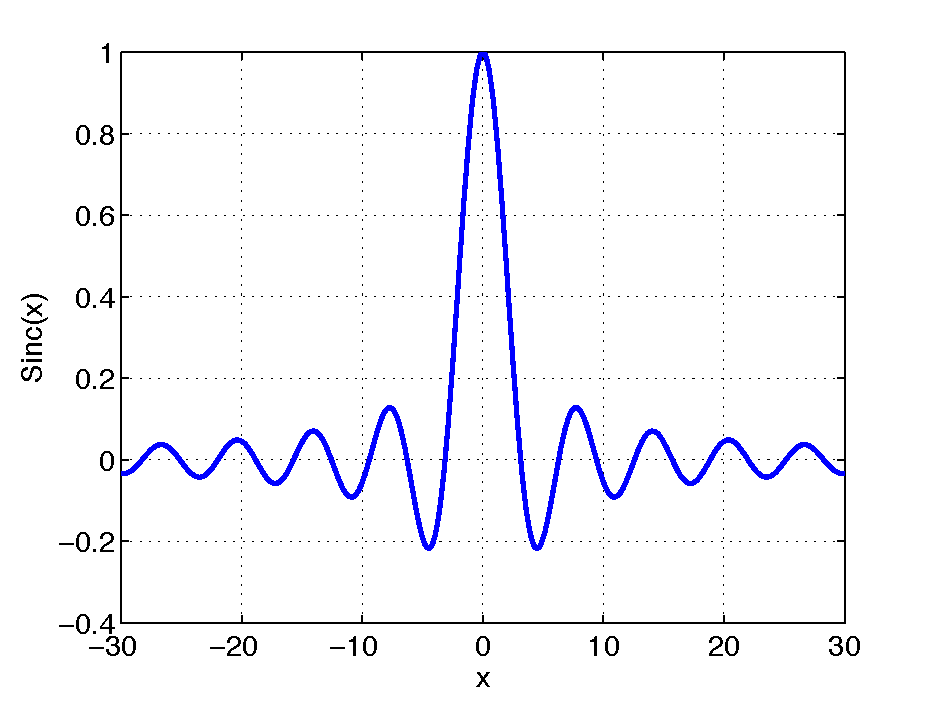
\includegraphics[width=.6\linewidth]{Figures/SincPlot}
%		\caption{Here goes the caption.}
%		\label{fig:Sinc}
%	\end{center}
%\end{figure}
%Figure~\ref{fig:Sinc} shows a shows a plot of the function $\sin(x)/x$. 
%
%If I need to make a simple diagram, I use powerpoint and select the drawing and save it as a pdf. For example, look at Figure~\ref{fig:MechaSys}.
%\begin{figure}[ht]
%	\begin{center}
%		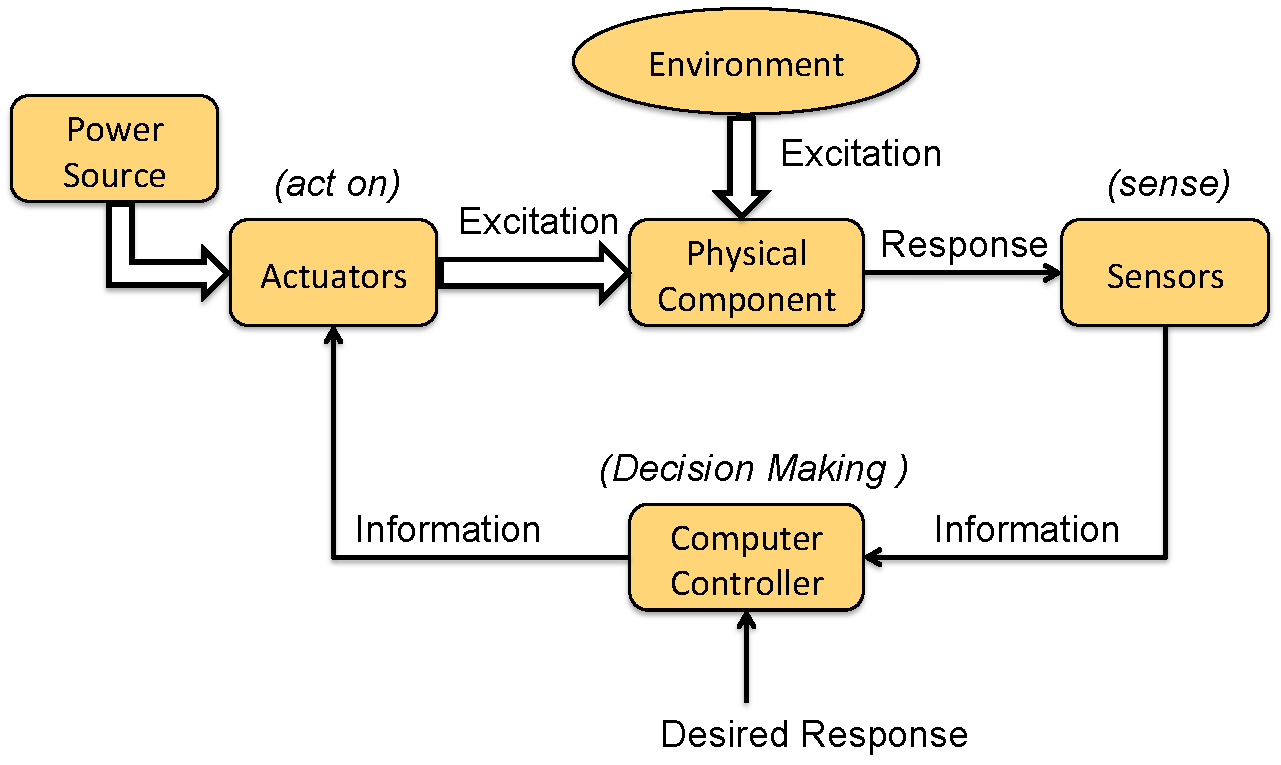
\includegraphics[width=.6\linewidth]{Figures/MechaSys}
%		\caption{Here goes the caption.}
%		\label{fig:MechaSys}
%	\end{center}
%\end{figure}
%
%
%To create lists use the environments \verb|itemize|, \verb|enumerate|, or \verb|description|
%
%The following is generated using \emph{itemize}
%\begin{itemize}
%	\item This is item 1 
%	\item This is item 2
%\end{itemize}
%%
%The following is generated using \emph{enumerate}
%\begin{enumerate}[1)]
%	\item This is item 1 
%	\begin{enumerate}[a)]
%		\item Subitem a
%		\item Subitem b
%		\begin{enumerate}[i)]
%			\item Subsubitem i
%			\item Subsubitem ii
%		\end{enumerate}
%	\end{enumerate}
%	\item This is item 2
%\end{enumerate}
%%
%The following is generated using \emph{description}
%\begin{description}
%	\item[foo)] This is item 1 
%	\item[bar)] This is item 2
%\end{description}
%
%
%
%To include a syntax-highlighted code listing, you can use the \emph{listings} package. The default options are specified by the \verb|\lstset| command. There are 3 main commands, all of which can include options to override the defaults:
%\begin{enumerate}
%	\item \verb|\lstinline|: Command for including code fragments inline with the text, as an alternative to \verb|\verb|. For example, we might describe function prototypes such as \lstinline[language=C,breaklines=true]|int main(int argc, char *argv[])|.
%	\item \verb|\begin{lstlisting}|,\ldots,\verb|\end{lstlisting}|: Environment for including a source code listing---embedded in the LaTeX source---in a box or floating environment. An example is shown in Listing~\ref{lst:sqrt}.
%	\item \verb|\lstinputlisting|: Command for including a source code listing---loaded from an external file---in a box or floating environment. This method is preferred over including the code source within the LaTeX file, since the code and its documentation can always be kept in sync. An example is shown in Listing~\ref{lst:matlabserial}.
%\end{enumerate}
%
%\begin{lstlisting}[
%language=C,
%float=h,
%numbers=none,
%xleftmargin=1cm,
%frame=none,
%caption={A winning entry from the 16th International Obfuscated C Code Contest, that computes the square root of its input.\label{lst:sqrt}}
%]
%#include <stdio.h>
%int l;int main(int o,char **O,
%int I){char c,*D=O[1];if(o>0){
%for(l=0;D[l              ];D[l
%++]-=10){D   [l++]-=120;D[l]-=
%110;while   (!main(0,O,l))D[l]
%+=   20;   putchar((D[l]+1032)
%/20   )   ;}putchar(10);}else{
%c=o+     (D[I]+82)%10-(I>l/2)*
%(D[I-l+I]+72)/10-9;D[I]+=I<0?0
%:!(o=main(c/10,O,I-1))*((c+999
%)%10-(D[I]+92)%10);}return o;}
%\end{lstlisting}
%
%\lstinputlisting[
%language=Matlab,
%float=h,
%numbers=left,
%xleftmargin=1cm,
%frame=shadowbox,
%caption={Matlab serial communication example.\label{lst:matlabserial}},
%morekeywords={try,catch}
%]{Code/serialtest.m}
%

\end{document}
